\documentclass[a3paper]{article}
\usepackage[a3paper]{geometry}
\usepackage[utf8]{inputenc}

% Math packages
\usepackage{amsmath,amsfonts,amssymb,amsthm}
\usepackage{mathrsfs}
\usepackage{thmtools}
\usepackage{array}
\usepackage{cleveref}
\usepackage{stmaryrd}
\usepackage{mathpartir}

% References
\usepackage{natbib}
\bibliographystyle{plainnat}

% Command control packages
\usepackage{ifthen}
\usepackage{ifpdf}

% Listings
\usepackage{listings}
\lstset{
  basicstyle=\ttfamily,
  columns=fullflexible,
  keepspaces=true,
  mathescape
}

% Rotate entire figures
\usepackage{rotating}

% Tikz
\usepackage{tikz}

%%% Comments
% Comments
\newcommand\lau[1]{{\color{purple} \sf \footnotesize {LS: #1}}\\}
\newcommand\dominique[1]{{\color{purple} \sf \footnotesize {DD: #1}}\\}
\newcommand\lars[1]{{\color{purple} \sf \footnotesize {LB: #1}}\\}

%%% Math environments
\declaretheorem[numbered=yes,name=Lemma,qed=$\blacksquare$]{lemma}
\declaretheorem[numbered=yes,name=Theorem,qed=$\blacksquare$]{theorem}
\declaretheorem[numbered=yes,name=Definition,qed=$\blacksquare$]{definition}
\declaretheorem[numbered=yes,name=Specification,qed=$\blacksquare$]{specification}


%%% Math notation
\newcommand{\defeq}{\stackrel{\textit{\tiny{def}}}{=}}
\newcommand{\defbnf}{::=}
\newcommand{\sem}[1]{\left\llbracket #1 \right\rrbracket}
\newcommand{\ssem}[2][\Phi]{\sem{#2}_{\mathrm{src}}(#1)}
\newcommand{\tsem}[2][\Phi]{\sem{#2}_{\mathrm{trg}}(#1)}
\newcommand{\dom}{\mathrm{dom}}
\newcommand{\powerset}[1]{\mathcal{P}(#1)}

\newcommand{\npair}[2][n]{\left(#1,#2\right)}

\newcommand{\nsubeq}[1][n]{\overset{#1}{\subseteq}}
\newcommand{\nsupeq}[1][n]{\overset{#1}{\supseteq}}

% Function arrows
\newcommand{\fun}{\rightarrow}
\newcommand{\parfun}{\rightharpoonup}

% Text
\newcommand{\tand}{\text{ and }}
\newcommand{\tor}{\text{ or }}
\newcommand{\totherwise}{\text{otherwise }}

% Equivalences
\newcommand{\sconeq}{\mathrel{\src{\approx_{\mathrm{ctx}}}}}
\newcommand{\tconeq}{\mathrel{\approx_{\mathrm{ctx}}}}

%%% Logical Relation notation
\newcommand{\typesetlr}[1]{\mathcal{#1}}
\newcommand{\lre}{\typesetlr{E}}
\newcommand{\lrk}{\typesetlr{K}}
\newcommand{\lrr}{\typesetlr{R}}
\newcommand{\lro}{\typesetlr{O}}
\newcommand{\lrv}{\typesetlr{V}}
\newcommand{\lrp}{\typesetlr{P}}
\newcommand{\lrm}{\typesetlr{M}}

\newcommand{\stpair}[3][]{
\ifthenelse{\equal{#1}{}}
{\left(\src{#2_S},#3_T\right)}
{\left(\src{#2},#3\right)}}


\newcommand{\memSat}[3][n]{#2 :_{#1}#3}

\newcommand{\World}{\mathrm{World}}
\newcommand{\RegionName}{\mathrm{RegionName}}
\newcommand{\Region}{\mathrm{Region}}
\newcommand{\spatial}{\mathrm{spatial}}
\newcommand{\spatialo}{\mathrm{spatial\_owned}}
\newcommand{\pure}{\mathrm{pure}}
\newcommand{\State}{\mathrm{State}}
\newcommand{\Rels}{\mathrm{Rels}}
\newcommand{\UPred}[1]{\mathrm(#1)}

\newcommand{\future}{\sqsupseteq}
\newcommand{\pub}{\mathrm{pub}}
\newcommand{\privft}{\future^{\priv}}
\newcommand{\pubft}{\future^{\pub}}


%%% Instruction formatting
\newcommand{\sourcecolortext}{blue}
\newcommand{\sourcecolor}{\color{blue}}
\newcommand{\src}[1]{{\sourcecolor #1}}
\newcommand{\targetcolortext}{black}
\newcommand{\targetcolor}[1]{\color{black}}
\newcommand{\trg}[1]{{\targetcolor{} #1}}

\newcommand{\zinstr}[1]{\texttt{#1}}
\newcommand{\oneinstr}[2]{
  \ifthenelse{\equal{#2}{}}
  {\zinstr{#1}}
  {\zinstr{#1} \; #2}
}
\newcommand{\twoinstr}[3]{
  \ifthenelse{\equal{#2#3}{}}
  {\zinstr{#1}}
  {\zinstr{#1} \; #2 \; #3}
}
\newcommand{\threeinstr}[4]{
  \ifthenelse{\equal{#2#3#4}{}}
  {\zinstr{#1}}
  {\zinstr{#1} \; #2 \; #3 \; #4}
}

\newcommand{\fourinstr}[5]{
  \ifthenelse{\equal{#2#3#4#5}{}}
  {\zinstr{#1}}
  {\zinstr{#1} \; #2 \; #3 \; #4 \; #5}
}


%%% Source language
% No arguments
\newcommand{\sfail}{\zinstr{\src{fail}}}
\newcommand{\shalt}{\zinstr{\src{halt}}}
\newcommand{\sreturn}{\zinstr{\src{return}}}

% One argument
\newcommand{\sjmp}[1]{\oneinstr{\src{jmp}}{#1}}
\newcommand{\spush}[1]{\oneinstr{\src{push}}{#1}}
\newcommand{\spop}[1]{\oneinstr{\src{pop}}{#1}}

% Two arguments
\newcommand{\sjnz}[2]{\twoinstr{\src{jnz}}{#1}{#2}}
\newcommand{\sisptr}[2]{\twoinstr{\src{gettype}}{#1}{#2}}
\newcommand{\sgeta}[2]{\twoinstr{\src{geta}}{#1}{#2}}
\newcommand{\sgetb}[2]{\twoinstr{\src{getb}}{#1}{#2}}
\newcommand{\sgete}[2]{\twoinstr{\src{gete}}{#1}{#2}}
\newcommand{\sgetp}[2]{\twoinstr{\src{getp}}{#1}{#2}}
%\newcommand{\sgetloc}[2]{\twoinstr{\src{getloc}}{#1}{#2}}
\newcommand{\sgetlin}[2]{\twoinstr{\src{get}}{#1}{#2}}
\newcommand{\smove}[2]{\twoinstr{\src{move}}{#1}{#2}}
\newcommand{\sstore}[2]{\twoinstr{\src{store}}{#1}{#2}}
\newcommand{\sload}[2]{\twoinstr{\src{load}}{#1}{#2}}
\newcommand{\scca}[2]{\twoinstr{\src{cca}}{#1}{#2}}
\newcommand{\ssload}[2]{\twoinstr{\src{sload}}{#1}{#2}}
\newcommand{\sxjmp}[2]{\twoinstr{\src{xjmp}}{#1}{#2}}
\newcommand{\ssetatob}[2]{\twoinstr{\src{seta2b}}{#1}{#2}}
% scall - special two instruction
\newcommand{\scall}[3][]{  
\ifthenelse{\equal{#2#3}{}}
  {\ensuremath{\zinstr{\src{call}}_{#1}}}
  {\ensuremath{\zinstr{\src{call}}_{#1} \; #2 \; #3}}
}


% Three arguments
\newcommand{\srestrict}[3]{\threeinstr{\src{restrict}}{#1}{#2}{#3}}
\newcommand{\slt}[3]{\threeinstr{\src{lt}}{#1}{#2}{#3}}
\newcommand{\splus}[3]{\threeinstr{\src{plus}}{#1}{#2}{#3}}
\newcommand{\sminus}[3]{\threeinstr{\src{minus}}{#1}{#2}{#3}}
\newcommand{\scseal}[3]{\threeinstr{\src{cseal}}{#1}{#2}{#3}}
\newcommand{\ssplice}[3]{\threeinstr{\src{splice}}{#1}{#2}{#3}}


% Four arguments
%\newcommand{\ssubseg}[4]{\fourinstr{\src{subseg}}{#1}{#2}{#3}{#4}}
\newcommand{\ssplit}[4]{\fourinstr{\src{split}}{#1}{#2}{#3}{#4}}

%%% Target language
% No arguments
\newcommand{\tfail}{\zinstr{\trg{fail}}}
\newcommand{\thalt}{\zinstr{\trg{halt}}}

% One argument
\newcommand{\tjmp}[1]{\oneinstr{\trg{jmp}}{#1}}

% Two arguments
\newcommand{\tjnz}[2]{\twoinstr{\trg{jnz}}{#1}{#2}}
\newcommand{\tisptr}[2]{\twoinstr{\trg{gettype}}{#1}{#2}}
\newcommand{\tgeta}[2]{\twoinstr{\trg{geta}}{#1}{#2}}
\newcommand{\tgetb}[2]{\twoinstr{\trg{getb}}{#1}{#2}}
\newcommand{\tgete}[2]{\twoinstr{\trg{gete}}{#1}{#2}}
\newcommand{\tgetp}[2]{\twoinstr{\trg{getp}}{#1}{#2}}
%\newcommand{\tgetloc}[2]{\twoinstr{\trg{getloc}}{#1}{#2}}
\newcommand{\tgetlin}[2]{\twoinstr{\trg{getl}}{#1}{#2}}
\newcommand{\tmove}[2]{\twoinstr{\trg{move}}{#1}{#2}}
\newcommand{\tstore}[2]{\twoinstr{\trg{store}}{#1}{#2}}
\newcommand{\tload}[2]{\twoinstr{\trg{load}}{#1}{#2}}
\newcommand{\tcca}[2]{\twoinstr{\trg{cca}}{#1}{#2}}
\newcommand{\txjmp}[2]{\twoinstr{\trg{xjmp}}{#1}{#2}}
\newcommand{\tsetatob}[2]{\twoinstr{\trg{seta2b}}{#1}{#2}}

% Three arguments
\newcommand{\tsplice}[3]{\threeinstr{\trg{splice}}{#1}{#2}{#3}}
\newcommand{\trestrict}[3]{\threeinstr{\trg{restrict}}{#1}{#2}{#3}}
\newcommand{\tlt}[3]{\threeinstr{\trg{lt}}{#1}{#2}{#3}}
\newcommand{\tplus}[3]{\threeinstr{\trg{plus}}{#1}{#2}{#3}}
\newcommand{\tminus}[3]{\threeinstr{\trg{minus}}{#1}{#2}{#3}}
\newcommand{\tcseal}[3]{\threeinstr{\trg{cseal}}{#1}{#2}{#3}}

% Four arguments
%\newcommand{\tsubseg}[4]{\fourinstr{\trg{subseg}}{#1}{#2}{#3}{#4}}
\newcommand{\tsplit}[4]{\fourinstr{\trg{split}}{#1}{#2}{#3}{#4}}

%%% Domains
\newcommand{\plaindom}[1]{\mathrm{#1}}

\newcommand{\nats}{\mathbb{N}}
\newcommand{\ints}{\mathbb{Z}}

%%% Updates
\newcommand{\update}[2]{[#1 \mapsto #2]}
\newcommand{\updReg}[2]{\update{\reg.#1}{#2}}
\newcommand{\updPc}[1]{\Phi\updReg{\pcreg}{#1}}

%%% Source dom
\newcommand{\shareddom}[1]{\mathrm{#1}}
\newcommand{\RegName}{\shareddom{RegisterName}}
\newcommand{\Addr}{\shareddom{Addr}}
\newcommand{\Seal}{\shareddom{Seal}}
\newcommand{\Perm}{\shareddom{Perm}}
\newcommand{\Caps}{\shareddom{Cap}}
\newcommand{\SealableCaps}{\shareddom{SealableCap}}
\newcommand{\Word}{\shareddom{Word}}
\newcommand{\Instr}{\shareddom{Instr}}
\newcommand{\Mem}{\shareddom{Memory}}
\newcommand{\Reg}{\shareddom{RegisterFile}}
\newcommand{\Stk}{\shareddom{Stack}}
\newcommand{\Conf}{\shareddom{Conf}}
\newcommand{\ExecConf}{\shareddom{ExecConf}}
%\newcommand{\Global}{\shareddom{Global}}
\newcommand{\Linear}{\shareddom{Linear}}
\newcommand{\MemSeg}{\shareddom{MemorySegment}}
\newcommand{\StkFrame}{\shareddom{StackFrame}}
\newcommand{\Stack}{\shareddom{Stack}}

\newcommand{\scbnf}{\shareddom{sc}}
\newcommand{\cbnf}{\shareddom{c}}
\newcommand{\permbnf}{\shareddom{perm}}
\newcommand{\addrbnf}{\shareddom{a}}
\newcommand{\basebnf}{\shareddom{base}}
\newcommand{\aendbnf}{\shareddom{end}}
\newcommand{\rbnf}{\shareddom{r}}
%\newcommand{\glbnf}{\shareddom{gl}}
\newcommand{\linbnf}{\shareddom{l}}
\newcommand{\sealbasebnf}{\sigma_\shareddom{base}}
\newcommand{\sealendbnf}{\sigma_\shareddom{end}}

\newcommand{\sstk}{\shareddom{stk}}
\newcommand{\smsstk}{\shareddom{ms_{stk}}}
\newcommand{\sstkframe}{\shareddom{frame}}
\newcommand{\sopc}{\shareddom{opc}}
\newcommand{\sastk}{\shareddom{a_{stk}}}
\newcommand{\perm}{\var{perm}}
%\newcommand{\gl}{\var{g}}
\newcommand{\lin}{\var{l}}
\newcommand{\base}{\shareddom{base}}
\newcommand{\aend}{\shareddom{end}}
\newcommand{\addr}{\shareddom{a}}
\newcommand{\scap}{\shareddom{c}}
\newcommand{\sms}{\shareddom{ms}}

\newcommand{\stkptr}[1]{\mathrm{stack\text{-}ptr}(#1)}
\newcommand{\retptr}{\mathrm{ret\text{-}ptr}}
\newcommand{\retptrd}{\mathrm{ret\text{-}ptr\text{-}data}}
\newcommand{\retptrc}{\mathrm{ret\text{-}ptr\text{-}code}}

\newcommand{\seal}[1]{\shareddom{seal}(#1)}
\newcommand{\sealed}[1]{\shareddom{sealed}(#1)}

\newcommand{\failed}{\mathrm{failed}}
% DOMI: defining a macro named ``undefined'' breaks many latex packages.
%       (this is just another way that LaTeX is broken as a programming language)
% \newcommand{\undefined}{\mathrm{undefined}}
\newcommand{\tundefined}{\mathrm{undefined}}
\newcommand{\halted}{\mathrm{halted}}

%%% Target domain
\newcommand{\targetdom}[1]{\mathrm{#1}}
\newcommand{\tRegName}{\targetdom{RegisterName}}

%%% Programs and contexts
\newcommand{\program}{\mathscr{P}}
\newcommand{\context}{\mathscr{C}}

\newcommand{\plug}[2]{#1[#2]}

%%% Operational semantics
\newcommand{\step}{\rightarrow}
\newcommand{\nstep}[1][n]{\step_{#1}}
\newcommand{\steps}{\step^*}
\newcommand{\diverge}{{\Uparrow}}
\newcommand{\term}[1][-]{{\Downarrow_{#1}}}

%%% Variables
\newcommand{\var}[1]{\mathit{#1}}
\newcommand{\rn}{\var{rn}}
\newcommand{\reg}{\var{reg}}
\newcommand{\mem}{\var{mem}}
\newcommand{\ms}{\var{ms}}
\newcommand{\pc}{\var{pc}}
\newcommand{\stk}{\var{stk}}
\newcommand{\link}{\var{link}}
\newcommand{\stkf}{\stk_{\var{frame}}}
\newcommand{\ret}{\var{ret}}
\newcommand{\data}{\var{data}}
\newcommand{\code}{\var{code}}
\newcommand{\priv}{\var{priv}}
\newcommand{\opc}{\var{opc}}
\newcommand{\odata}{\var{odata}}
\newcommand{\vsc}{\var{sc}}
\newcommand{\cb}{\var{cb}}
\newcommand{\baddr}{\var{b}}
\newcommand{\eaddr}{\var{e}}
\newcommand{\aaddr}{\var{a}}
\newcommand{\stdrng}{[\baddr,\eaddr]}

%%% Constants
\newcommand{\constant}[1]{\mathrm{#1}}
\newcommand{\calllen}{\constant{call\_len}}
\newcommand{\stkb}{\constant{stk\_base}}

%%% Named registers
\newcommand{\pcreg}{\mathrm{pc}}
\newcommand{\rstk}{\mathrm{r}_\mathrm{stk}}
\newcommand{\rO}{\mathrm{r}_\mathrm{ret}}
\newcommand{\rret}{\rO}
\newcommand{\rretc}{\mathrm{r}_\mathrm{ret code}}
\newcommand{\rretd}{\mathrm{r}_\mathrm{ret data}}
\newcommand{\rdata}{\mathrm{r}_\mathrm{data}}

%%% locality
%\newcommand{\plainlocality}[1]{\mathrm{#1}}
%\newcommand{\glob}{\plainlocality{global}}
%\newcommand{\local}{\plainlocality{local}}

%%% linearity
\newcommand{\plainlinearity}[1]{\mathrm{#1}}
\newcommand{\linear}{\plainlinearity{linear}}
\newcommand{\normal}{\plainlinearity{normal}}


%%% Permissions
\newcommand{\plainperm}[1]{\textsc{#1}}
%\newcommand{\rwlx}{\plainperm{rwlx}}
\newcommand{\rwx}{\plainperm{rwx}}
\newcommand{\rx}{\plainperm{rx}}
%\newcommand{\rwlxo}{\plainperm{rwlxo}}
%\newcommand{\rwlo}{\plainperm{rwlo}}
%\newcommand{\rwl}{\plainperm{rwl}}
%\newcommand{\rwxo}{\plainperm{rwxo}}
%\newcommand{\rwo}{\plainperm{rwo}}
\newcommand{\rw}{\plainperm{rw}}
%\newcommand{\rxo}{\plainperm{rxo}}
\newcommand{\readonly}{\plainperm{r}}
\newcommand{\ro}{\readonly}
\newcommand{\noperm}{\plainperm{0}}
%\newcommand{\nopermo}{\plainperm{0o}}
%\newcommand{\enter}{\plainperm{e}}
%\newcommand{\entero}{\plainperm{eo}}

%%% Braces
\newcommand{\comp}[1]{[#1]}

%%% Functions
\newcommand{\plainfun}[2]{
  \ifthenelse{\equal{#2}{}}
  {\mathit{#1}}
  {\mathit{#1}(#2)}
}

%\newcommand{\isLoc}[1]{\plainfun{isLocal}{#1}}
%\newcommand{\nonLoc}[1]{\plainfun{nonLocal}{#1}}
%\newcommand{\opaquePerm}[1]{\plainfun{opaquePerm}{#1}}
%\newcommand{\updPcPerm}[1]{\plainfun{updatePcPerm}{#1}}
%\newcommand{\writeLocalAllowed}[1]{\plainfun{writeLocalAllowed}{#1}}
\newcommand{\addressable}[1]{\plainfun{addressable}{#1}}
\newcommand{\callCond}[1]{\plainfun{callCondition}{#1}}
\newcommand{\decInstr}[1]{\plainfun{decodeInstruction}{#1}}
\newcommand{\decPerm}[1]{\plainfun{decodePerm}{#1}}
\newcommand{\encInstr}[1]{\plainfun{encodeInstruction}{#1}}
\newcommand{\encPerm}[1]{\plainfun{encocePerm}{#1}}
\newcommand{\encType}[1]{\plainfun{encodeType}{#1}}
\newcommand{\exec}[1]{\plainfun{executable}{#1}}
\newcommand{\execCond}[1]{\plainfun{executeCondition}{#1}}
\newcommand{\isLinear}[1]{\plainfun{isLinear}{#1}}
\newcommand{\linCons}[1]{\plainfun{linearityConstraint}{#1}}
\newcommand{\noRetStkMs}[1]{\plainfun{noRetStk_{ms}}{#1}}
\newcommand{\noRetStkReg}[1]{\plainfun{noRetStk_{reg}}{#1}}
\newcommand{\nonExec}[1]{\plainfun{nonExecutable}{#1}}
\newcommand{\nonLinear}[1]{\plainfun{nonLinear}{#1}}
\newcommand{\nonZero}[1]{\plainfun{nonZero}{#1}}
\newcommand{\range}[1]{\plainfun{range}{#1}}
\newcommand{\readAllowed}[1]{\plainfun{readAllowed}{#1}}
\newcommand{\readCond}[1]{\plainfun{readCondition}{#1}}
\newcommand{\writeCond}[1]{\plainfun{writeCondition}{#1}}
\newcommand{\sealAss}[1]{\plainfun{sealAssignment}{#1}}
\newcommand{\updPcAddr}[1]{\plainfun{updatePc}{#1}}
\newcommand{\withinBounds}[1]{\plainfun{withinBounds}{#1}}
\newcommand{\writeAllowed}[1]{\plainfun{writeAllowed}{#1}}


\title{Technical Report}

\begin{document}
\maketitle
\tableofcontents
\section{The two capability machines}
\subsection{Domains}
\label{sec:domains}

% \dominique{7-9-2017: Should we keep local/global and linear/non-linear?  I was thinking just the latter would suffice...}
% \lau{07-09-2017: The local/global mechanism still has some value as it now can be used for the purpose of arguments that cannot be stored by the receiver (if you are willing to ``pay'' the clearing cost). I do, however, not think that it is strictly necessary here to make things work.}
% \lau{12-09-2017: I will remove the local capabilities today for the reasons we have discussed (they add to the complexity and they seem to be of little to no use without a clear memory instruction).}
Source language domains:
\[
  \begin{array}{rrcl}
   \addrbnf,\basebnf \in & \Addr & \defeq & \nats \\
    \sealbasebnf, \sigma \in & \Seal & \defeq & \nats \\
    &\Word & \defeq & \ints \uplus \SealableCaps\\
    \permbnf \in& \Perm & \defbnf & \dots \\
    &\linbnf & \defbnf & \linear \mid \normal \\
    &\aendbnf & \in & \Addr \uplus \{\infty \} \\
    &\sealendbnf & \in & \Seal \uplus \{\infty \} \\
    &\scbnf &\defbnf & ((\permbnf,\linbnf),\basebnf,\aendbnf,\addrbnf) \mid \seal{\linbnf,\sealbasebnf,\sealendbnf,\sigma}\\
    & & & {\sourcecolor{} \mid \stkptr{\permbnf,\basebnf,\aendbnf,\addrbnf}}\\ 
    &\cbnf & \defbnf &  \scbnf \mid \sealed{\scbnf,\sigma}{\sourcecolor{} \; \mid \retptrd(\sigma,(\basebnf,\aendbnf)) \mid \retptrc(\sigma,(\permbnf,\linbnf,\basebnf,\aendbnf,\addrbnf))}\\ 
    &\rbnf & \defbnf &\pcreg \mid \rret \mid \rstk \mid \rdata \mid \dots \\
    &\Reg & \defeq & \RegName \fun \Word\\
    &\Mem & \defeq & \Addr \fun \Word \\
    &\MemSeg & \defeq & \Addr \parfun \Word \\
    {\sourcecolor \sstkframe \in} & {\sourcecolor \StkFrame} & {\sourcecolor \defeq} & {\sourcecolor \Caps \times \MemSeg \times \Addr}\\
    \src{\sstk \in}& \src{ \Stack} & \src{ \defeq} & \src{ \StkFrame^*} \\
    \Phi \in & \ExecConf & \defeq & \Mem \times \Reg {\sourcecolor{} \; \times \; \Stack \times \MemSeg }\\
    &\Conf & \defeq & \ExecConf \uplus \{\failed\} \uplus (\{\halted\} \times \Mem)
  \end{array}
\]
\lau{06-09-2017: Should seals also have the option to be linear?}
\lau{13-09-2017: For now I have added linearity to the seals.}
\dominique{27-9-2017: I think we should have versions of $\retptrd$ and $\retptrc$ for non-top stack frames and define that invoking them with the current stack pointer will fail.}
\lau{28-09-2017: Why would you like this? If we want to add this, we will have to be careful, because an old code-return-pointer may fit perfectly well with our new data-return-pointer, so in this case it should not fail. We added the seal to the return pointers, so we had some way of figuring out whether two return pointers would actually fit together.}
\dominique{27-9-2017: Likewise, I think we need to have a source-language representation for a pointer into one of the non-top stack frames, as we may need to be able to back-translate adversary code that reads/writes in those.}
\lau{28-09-2017: At the moment, the only part of the stack that is stored in the stack frame is the private part. Specifically it is the part from the base to the current address of the stack pointer \emph{in $r_\stk$}. This means that if someone saves a stack pointer, so it is not included in the call, then they can still use it because that part of the stack was not encapsulated in a stack frame. Makes sense?}
The target language domains are all the non blue parts in the above. The source language domains are the black and blue parts in the above. Further
\begin{itemize}
\item $\linbnf$ defines domain $\Linear$
\item $\scbnf$ defines domain $\SealableCaps$
\item $\cbnf$ defines domain $\Caps$
\item $\rbnf$ defines the finite set $\RegName$.
\item $\Perm$ is defined as the set of permissions in Figure~\ref{fig:perm-hier}.
\end{itemize}

In the source language, $\src{\Stack}$ is a call stack that contains the data for each call. The call stack consists of a number of $\src{\StkFrame}$'s that contains 1) the old pc, 2) caller's private stack, and 3) the address of the old stack pointer. 

 In both languages, the base address of the stack is known (the stack grows downwards in memory, so the base address marks the end of the stack). In the target language, this will be the base address of some linear capability. The base address can be any address on the machine, but it will have to remain the same. We write this constant as
\[
  \stkb
\]

More convenient definitions
\[
  \begin{array}{rcl}
    \Phi(r) & \defeq & \Phi.\reg(r)
  \end{array}
\]
where $r\in \RegName$.

\subsubsection{Useful definitions}
\begin{definition}
  For a capability $c=((\_,\_),\baddr,\eaddr,\_)$ we say it has range $[\baddr,\eaddr]$ and we define
  \[
    \range{c} = [\baddr,\eaddr]
  \]
  Similarly for seals and stack pointers:
  \[
    \range{\seal{\_,\sigma_\baddr,\sigma_\eaddr,\_}} = [\sigma_\baddr,\sigma_\eaddr]
  \]
  and
  \[
    \src{\range{\stkptr{\_,\baddr,\eaddr,\_}} = [\baddr,\eaddr]}
  \]
\end{definition}

\subsection{Syntax}
\label{sec:syntax}
The target machine is a simple capability machine with memory capabilities and sealed capabilities\footnote{In previous work, we used enter capabilities but for this the complexity introduced by mixing writable and executable memory is difficult to handle.} (inspired by CHERI). The syntax of the instructions of the target machine is defined as follows:
\[
\begin{array}{rcl}
n &\in & \nats \\
\trg{r} &\in &  \tRegName \\
\trg{\rn} &\defbnf &  \trg{r} \mid n \\
\trg{i} &\defbnf & \tfail \mid \thalt \mid \tjmp{\trg{r}} \mid \tjnz{\trg{r}}{\trg{\rn}} \mid \tisptr{\trg{r}}{\trg{r}} \mid \tgeta{\trg{r}}{\trg{r}} \mid \tgetb{\trg{r}}{\trg{r}} \mid \\
      & &  \tgete{\trg{r}}{\trg{r}}\mid \tgetp{\trg{r}}{\trg{r}} \mid \tgetlin{\trg{r}}{\trg{r}} \mid \tmove{\trg{r}}{\trg{\rn}} \mid \tstore{\trg{r}}{\trg{r}} \mid\\
      & &  \tload{\trg{r}}{\trg{r}} \mid \tcca{\trg{r}}{\trg{\rn}} \mid \trestrict{\trg{r}}{\trg{r}}{\trg{\rn}} \mid \tlt{\trg{r}}{\trg{r}}{\trg{r}} \mid \\
  & & \tplus{\trg{r}}{\trg{\rn}}{\trg{\rn}} \mid \tminus{\trg{r}}{\trg{\rn}}{\trg{\rn}} \mid \tsetatob{\trg{r}}{\trg{r}} \mid \txjmp{\trg{r}}{\trg{r}} \mid \tcseal{\trg{r}}{\trg{r}}{\trg{r}} \mid \\ 
      & &   \tsplit{\trg{r}}{\trg{r}}{\trg{r}}{\trg{\rn}} \mid\tsplice{\trg{r}}{\trg{r}}{\trg{r}} 
\end{array}
\]
$i$ defines the set $\Instr$

The source machine is also a capability machine with memory capabilities and sealed capabilities. Unlike the target machine, the source machine is going to have a built in stack along with special stack and return capabilities. The syntax of the source machine language is as follows:
\[
  \begin{array}{rcl}
    n & \in & \nats \\
    \src{r} &\in &  \RegName\\
    \src{\rn} &\defbnf & \src{r} \mid n \\
    \src{i} & \defbnf &  \trg{i} \mid \scall{\src{r}}{\src{r}}
  \end{array}
\]
There is one syntactic difference between the source language and the target language, namely the target language has an extra instruction in the $\scall{}{}$ instruction.

The source machine allows for variable length instructions which we utilize for $\scall{}{}$. In other words, when we $\scall{}{}$ is decoded, a series of addresses in memory must contain what corresponds to the call instruction. This is described in more detail when we present the decoding function.

\subsection{Permissions}
\lau{23-03-2017: I am not sure we need the opaque capabilities anymore.} % I am not sure why I did not think the opaque capabilities where necessary, but I have a feeling we talked about this in Leuven and came to the conclusion that they were necessary.
\begin{figure}[!h]
  \centering
  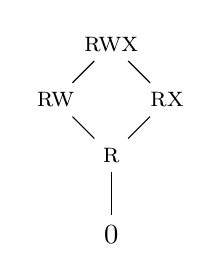
\begin{tikzpicture}[main node/.style={}]
    \node[main node] (rwx) {$\rwx$};
    \node[main node] (rx) [below right of=rwx] {$\rx$};

    \node[main node] (rw) [below left of=rwx,] {$\rw$};
    \node[main node] (r) [below right of=rw] {$\readonly$};
    \node[main node] (0) [below of=r] {$\noperm$};

    \path[every node/.style={font=\sffamily\small}]

    (rw) edge (r)
    (r) edge (0)

    (rwx) edge (rx)

    (rw) edge (rwx)
    (r) edge (rx);
  \end{tikzpicture}

  \caption{Permission hierarchy}
  \label{fig:perm-hier}
\end{figure}
\lau{01-09-2017: For now, I will add the linear capabilities such that a linear capability stays linear. It does, however, seem like it would be okay to have linear capabilities become non-linear (I at least don't see anything that would break down completely). One draw back would be that one could ``ruin'' the stack capability by making it non-linear.}
\dominique{7-9-2017: Err... you mean that we could allow non-linear capabilities to be made linear, right?  We definitely do not want to allow the stack or return capability to be made non-linear, as we want to prevent it from being aliased.}
\lau{07-09-2017: I actually did mean linear to non-linear (non-linear to linear does not make sense because the non-linear capability may have aliases). The operation that makes a linear capability non-linear would have to clear said capability. If a linear capability has been made non-linear, then someone who expects a linear capability can observe this difference and behave accordingly, i.e., fail the execution. It will, however, remain an invariant that there are no aliases for linear capabilities.}
\lau{07-09-2017: I had forgotten that return capabilities probably need to be linear. This would call for a ``load from offset'' operation to be able to load an in code stored seal (see the figure I drew about linking/seals).}
\lau{13-09-2017: Note that most of the above discussion is now captured in Section~\ref{sec:linear-cap}}

We assume functions $\decPerm{}$ and $\encPerm{}$.
\lau{15-09-2017: TODO, write more about these. Should be like in the local cap setting.}

\subsection{Operational Semantics}
\subsubsection{Notes}
Generally:
\begin{itemize}
%\item Opaque capabilities: Only allow locality and permission to be inspected (i.e., no addresses disclosed).
\item Linear capabilities are cleared when they move around in memory.
\end{itemize}

Source language:
\begin{itemize}
\item Variable length instructions that match the length of the compiled instructions
  \begin{itemize}
%  \item Opaque capabilities do not hide the length of a program (especially an issue if we ever hope to have error recovery).
  \item This is needed for correctness. See subsection~\ref{subsec:capability-opacity} for an example it helps prevent.
  \end{itemize}
\item Programs have undefined behavior when passing ret/stk pointers.
\end{itemize}

\dominique{27-09-2017: I think we need to do something about tail calls in the source language?}
\lau{27-09-2017: In what sense? Do you want to allow them (I do not think they are allowed at the moment?)}
\dominique{8-11-2017: Yes, I would like to support them.  I think it would be a strength of our calling convention that we can support them (as I expect we can) and it would be good to demonstrate this.}

Target language:
\begin{itemize}
\item 
\end{itemize}

\subsubsection{Step relations}
\paragraph{Decode and encode functions}
We assume functions $\decInstr{} : \Word \fun \Instr$ and $\encInstr{} : \Instr \fun \ints$ where $\Instr$ is the set of target level instructions.

The $\decInstr{}$ function must be surjective and injective for all non-$\tfail$ instructions. The $\encInstr{}$ function must be injective. Further $\decInstr{}$ must be the left inverse of $\encInstr{}$ that is for all $i \in \Instr$
\[
  \decInstr{}(\encInstr{i}) = i
\]

These functions are used for both the target and source level machine. When we write instructions in places where words are required, we will assume that $\encInstr{}$ is implicit.

\paragraph{Step relation}
The instruction $\scall{}{}$ has length $\calllen$ which means that it does not fit on one memory address. In fact, $\scall{}{}$ should be seen as a different way of interpreting a series of instruction rather than an instruction on its own. We therefore introduce $\scall[1]{r_1}{r_2},\dots,\scall[\calllen-1]{r_1}{r_2}$ as aliases for the instructions that constitute $\scall{r_1}{r_2}$ (see Paragraph~\ref{par:call-impl} for details). We define the following condition that indicates that $\aaddr$ is the first address of a $\scall{r_1}{r_2}$ instruction in the configuration $\Phi$:
\[
  \sourcecolor\left.
    \callCond{\Phi,r_1,r_2,\aaddr} = \left\{
      \begin{array}{l}
        \Phi.\mem(\aaddr) = \scall[1]{r_1}{r_2} \tand\\
        \vdots \\
        \Phi.\mem(\addr+\calllen-1) = \scall[\calllen]{r_1}{r_2}
      \end{array}
      \right.
  \right.
\]

We use the following step relation:

\begin{align*}
  \src{\Phi} & \; \src{\step \sem{\scall{r_1}{r_2}}(\Phi)} &  &\sourcecolor\left.\arraycolsep=0pt
                                                  \begin{array}[t]{l}
                                                    \text{if }\Phi(\pcreg) = ((\perm,\_),\baddr,\eaddr,\aaddr) \tand \\
                                                    \callCond{\Phi,r_1,r_2,\aaddr} \tand\\
                                                    \baddr \leq \aaddr \tand \aaddr + \calllen-1 \leq \eaddr \tand \\
                                                    \exec{\Phi(\pcreg)}
                                                  \end{array}\right.\\
  \Phi & \step \sem{\decInstr{\Phi.\mem(\aaddr)}}(\Phi) & &\left.\arraycolsep=0pt
                                                  \begin{array}[t]{l}
                                                    \text{if }\Phi(\pcreg) = ((\perm,\_),\baddr,\eaddr,\aaddr) \tand \\
                                                    \src{(\neg\callCond{\Phi,r_1,r_2,\aaddr} \tor}\\
                                                    \src{\eaddr < \aaddr + \calllen-1) \tand} \\
                                                    \baddr \leq \aaddr \leq \eaddr\tand\\
                                                    \exec{\Phi(\pcreg)}
                                                  \end{array}\right.\\
  \Phi& \step \failed & & \totherwise
\end{align*}

\paragraph{Call implementation}
\label{par:call-impl}
\lau{16-10-2017: Fill this paragraph with $\scall{}{}$ implementation, i.e., the instructions $\scall[1]{r_1}{r_2} \dots \scall[\calllen]{r_1}{r_2}$ is equal to. Add convenience notation like $\update{\mem.a}{\scall{r_1}{r_2}} = \dots$}
\lau{16-10-2017: Implementation of $\scall{}{}$ may need registers for temporary registers - we should update the semantics accordingly.}
\[
  \begin{array}{l}
    \text{// push current end address of stack pointer on the stack.}\\
    \tgete{r_{t1}}{\rstk}\\
    \tstore{\rstk}{r_{t1}}\\
    \tcca{\rstk}{-1}\\
    \text{// split the stack at its current address.}\\
    \tgeta{r_{t1}}{\rstk}\\
    \tsplit{\rstk}{\rretd}{\rstk}{r_{t1}}\\
    \text{// load the seal for the return pointer through the pc capability.}\\
    \tmove{r_{t1}}{\pcreg}\\
    \tsetatob{r_{t1}}{r_{t1}}\\
    \tload{r_{t1}}{r_{t1}}\\
    \tcca{r_{t1}}{{\color{red} \dots}}\\
    // \text{seal the used stack frame as the data part of the return pointer pair.}\\
    \tcseal{\rretd}{\rretd}{r_{t1}}\\
    // \text{obtain the code part of the return pointer pair and seal it too.}\\
    \tmove{\rretc}{\pcreg}\\
    \tcca{\rretc}{5} \text{ //magic number is offset to return code}\\
    \tcseal{\rretc}{\rretc}{r_{t1}}\\
    // \text{now clear temporary register and jump to the adversary.}\\
    \tmove{r_{t1}}{0}\\
    \txjmp{r_1}{r_2}\\
    \text{// the following is the return code}\\
    \text{// check that the stack pointer is the same we handed out.}\\
    \tgetb{r_{t1}}{\rstk}\\
    \tminus{r_{t1}}{t_{t1}}{\stkb} \text{ //$\stkb$ is the stack base constant} \\
    \tmove{r_{t2}}{\pcreg}\\
    \tcca{r_{t2}}{5} \text{ //magic number is the offset to fail} \\
    \tjnz{r_{t2}}{r_{t1}} \\
    \tcca{r_{t2}}{1} \text{ //magic number is the offset to after fail} \\
    \tjmp{r_{t2}} \\
    \tfail \\
    \text{// join our stored private stack frame with the rest of the stack}\\
    \tsplice{\rstk}{\rstk}{\rdata} \\
    \text{// pop the stored stack end address}\\
    \tcca{\rstk}{1}\\
    \text{// clear temporary registers used}\\
    \tmove{r_{t1}}{0}\\
    \tmove{r_{t2}}{0}\\
    \text{// continue program after invocation.}
  \end{array}
\]
\dominique{Return code could be simplified if we had jz in addition to jnz.}
\dominique{It is a bit annoying that we store the stack end address before invocation if we do not use it.
  I understand this is for ensuring that our private stack frame is not empty, which is important.
  But why don't we just push a constant then?
  Also: perhaps we could only do it if the current private stack frame is empty to begin with?
}
{\color{red} \dots} needs to be the offset to the seal we want to use.
The call code does the following:
\begin{itemize}
\item Store the end address of the stack to the stack (this ensures the stack is non-empty), and decrement the pointer according to convention.
\item Get the current address of the stack pointer and split according to it.
\item Retrieve the seal of the program.
\item cca the seal, so the seal to be used is active 
\item seal our private part of the stack capability.
\item Move the pc out of the pc register, adjust it to point to the first address of the return code, and seal it.
\item clear the temporary register.
\item cross jump to the two specified registers.
\item Upon return:
  \begin{itemize}
  \item get the base of the stack and check that it matches up with the global base of the stack.If not, fail.
  \item splice the returned stack pointer and the stack pointer for our private stack.
  \item adjust stack pointer to first empty address (the address with the end address is considered free)  
  \item clear the temporary registers.
  \end{itemize}
\end{itemize}

\subsubsection{Helpful functions and sets}


\[
  \updPcAddr{c} \defeq \dots
\]

\[
  \readAllowed{} \defeq \dots
\]

\[
  \writeAllowed{} \defeq \dots
\]

\[
  \isLinear{\cb} \defeq
  \begin{cases}
    \top & 
    \arraycolsep=0pt
    \begin{array}[t]{l}
      \cb = ((\_,\linear),\_,\_,\_) \tor\\
      \cb = \seal{\linear,\_,\_,\_} \tor\\
      \cb = \sealed{\cb',\_} \tand \isLinear{\cb'} 
    \end{array}\\
    \src{\top} & 
    \sourcecolor\left.
    \arraycolsep=0pt
    \begin{array}[t]{l}
      \cb = \stkptr{\_,\_,\_,\_}\\
      \cb = \retptrd(\_,\_)
    \end{array}\right.\\
    \bot & \totherwise
  \end{cases}
\]

\[
  \nonLinear{\cb} \defeq \neg \isLinear{\cb}
\]

\[
  \linCons{w} \defeq
  \begin{cases}
    0 & \isLinear{w} \\
    w & \totherwise
  \end{cases}
\]

\[
  \exec{\cb} \defeq \dots
\]

\[
  \nonExec{\cb} \defeq \dots
\]

\[
  \withinBounds{c} \defeq \dots
\]

\[
  \nonZero{w} \defeq
  \begin{cases}
    \bot & w \in \ints \tand w = 0 \\
    \top & \totherwise
  \end{cases}
\]

\subsubsection{Step Relation}

\subsubsection{Instruction Interpretation}
We have unified the two languages in the below definitions. Everything written in black is common for both source and target language. Everything written in \src{blue} is specific to the source language.

\noindent\textbf{fail and halt}\\
\begin{align*}
  \sem{\tfail}(\Phi) = & \; \failed \\
  \sem{\thalt}(\Phi) = & \; (\halted, \Phi.\mem)
\end{align*}

\noindent\textbf{jmp and jnz}\\
\begin{align*}
  \sem{\tjmp{r}}(\Phi) = &  
                     \begin{cases}
                       \Phi\updReg{r}{w}\updReg{\pcreg}{\Phi(r)} & w = \linCons{\Phi(r)}
                     \end{cases}
\end{align*}

\begin{align*}
  \sem{\tjnz{r}{\rn}}(\Phi) = &       
                             \begin{cases}
                               \arraycolsep=0pt
                               \begin{array}[t]{rl}
                                 \Phi&\updReg{r}{w}\\
                                     &\updReg{\pcreg}{\Phi(r)}
                               \end{array}
                                               & w = \linCons{\Phi(r)} \tand \nonZero{\Phi(\rn)}\\
                               \updPcAddr{\Phi} & \totherwise
                             \end{cases}
\end{align*}

\noindent\textbf{gettype}\\
In the definitions of the semantics below, we use a function $\encType{} : \Word \rightarrow \ints$. This is an encoding function for which the specific implementation does not matter. As the words of the two machines differ, we really need two functions which we call $\encType{}_{\var{src}}$ and $\encType{}_{\var{trg}}$. These two functions need to be related in the following way:
\lau{14-09-2017: Insert the relation. My impression is that the the words specific to the source machine should have the same "type" as their implementation at the source level (I am not sure this is the case - maybe it is okay to just relate the values returned by the special words to the ones returned when used with the implementation). }
\dominique{20-9-2017: I also think gettype for source-specific words should produce the same result than gettype for their implementation.}
\begin{align*}
  \sem{\tisptr{r_1}{r_2}}(\Phi) = & \; \updPcAddr{}(\Phi\updReg{r_1}{\encType{\Phi(r_2)}})
\end{align*}


\noindent\textbf{geta, getb, gete, getp, and getl}\\
We assume function to encode and decode permissions as well as a function to encode and decode linearity. The functions are used implicitly when a permission or linearity is used in a place where they need to be a word.
\lau{14-09-2017: Write more about this (types and assumptions)}
\begin{align*}
  \sem{\tgeta{r_1}{r_2}}(\Phi) = & 
                                   \begin{cases}
                                     \updPcAddr{\Phi\updReg{r_1}{\aaddr}} & 
                                     \arraycolsep=0pt
                                     \begin{array}[t]{l}
                                       \Phi(r_2) = ((\_,\_),\_,\_,\aaddr) \\
                                       \quad \tor \Phi(r_2) = \seal{\_,\_,\_,\aaddr} \\
                                       \quad \src{\tor \Phi(r_2) = \stkptr{\_,\_,\_,\aaddr} } \\
                                     \end{array} \\
                                     \updPcAddr{\Phi\updReg{r_1}{-1}} & \totherwise
                                   \end{cases}
\end{align*}

\begin{align*}
  \sem{\tgetb{r_1}{r_2}}(\Phi) = & 
                                   \begin{cases}
                                     \updPcAddr{\Phi\updReg{r_1}{\baddr}} & 
                                     \arraycolsep=0pt
                                     \begin{array}[t]{l}
                                       \Phi(r_2) = ((\_,\_),\baddr,\_,\_) \\
                                       \quad \tor \Phi(r_2) = \seal{\_,\baddr,\_,\_} \\
                                       \quad \src{\tor \Phi(r_2) = \stkptr{\_,\baddr,\_,\_} } \\
                                     \end{array} \\
                                     \updPcAddr{\Phi\updReg{r_1}{-1}} & \totherwise
                                   \end{cases}
\end{align*}

\begin{align*}
  \sem{\tgete{r_1}{r_2}}(\Phi) = & 
                                   \begin{cases}
                                     \updPcAddr{\Phi\updReg{r_1}{\eaddr}} & 
                                     \arraycolsep=0pt
                                     \begin{array}[t]{l}
                                       \Phi(r_2) = ((\_,\_),\_,\eaddr,\_) \\
                                       \quad \tor \Phi(r_2) = \seal{\_,\_,\eaddr,\_} \\
                                       \quad \src{\tor \Phi(r_2) = \stkptr{\_,\_,\eaddr,\_} } \\
                                     \end{array} \\
                                     \updPcAddr{\Phi\updReg{r_1}{-1}} & \totherwise
                                   \end{cases}
\end{align*}
\lau{15-09-2017: Should gete and getb do something for seals?}

\begin{align*}
  \sem{\tgetp{r_1}{r_2}}(\Phi) = & 
                                   \begin{cases}
                                     \updPcAddr{\Phi\updReg{r_1}{\perm}} & 
                                     \arraycolsep=0pt
                                     \begin{array}[t]{l}
                                       \Phi(r_2) = ((\perm,\_),\_,\_,\_) \\
                                       \quad \src{\tor \Phi(r_2) = \stkptr{\perm,\_,\_,\_} } \\
                                     \end{array} \\
                                     \updPcAddr{\Phi\updReg{r_1}{-1}} & \totherwise
                                   \end{cases}
\end{align*}

\begin{align*}
  \sem{\tgetlin{r_1}{r_2}}(\Phi) = & 
                                   \begin{cases}
                                     \updPcAddr{\Phi\updReg{r_1}{\lin}} & 
                                     \arraycolsep=0pt
                                     \begin{array}[t]{l}
                                       \Phi(r_2) = ((\_,\lin),\_,\_,\_) \\
                                       \quad \tor \Phi(r_2) = \seal{\lin,\_,\_,\_} \\
                                       \quad \src{\tor \Phi(r_2) = \stkptr{\_,\_,\_,\_} \tand l = \linear}\\
                                     \end{array} \\
                                     \updPcAddr{\Phi\updReg{r_1}{-1}} & \totherwise
                                   \end{cases}
\end{align*}
\lau{15-09-2017: Should getl do something for seals?}
\lau{15-09-2017: Do we want to allow getl and getp to work on sealed capabilities?}

\noindent\textbf{move}\\
\begin{align*}
  \sem{\tmove{r}{\rn}}(\Phi) = & 
                              \begin{cases}
                                \updPcAddr{\Phi\updReg{r}{\rn}} & \rn \in \ints \\
                                \updPcAddr{\Phi\updReg{\rn}{w}\updReg{r}{\Phi(\rn)}} & w = \linCons{\Phi(\rn)}
                              \end{cases}
\end{align*}
Notice that in the case where we are moving a linear capability and $r = \rn$ the order of the updates matter.

\noindent\textbf{store}\\
\begin{align*}
  \sem{\tstore{r_1}{r_2}}(\Phi) = &
                                    \begin{cases}
                                      \updPcAddr{}\left(
                                        \arraycolsep=0pt
                                        \begin{array}{rl}
                                          \Phi&\updReg{r_2}{w_2}\\
                                              &\update{\mem.a}{w}
                                        \end{array}
\right) & 
                                      \arraycolsep=0pt
                                      \begin{array}[t]{l}
                                        \Phi(r_1) = ((\perm,\lin),\baddr,\eaddr,\aaddr) \tand \\
                                        \perm \in \writeAllowed{} \tand\\
                                        \withinBounds{\Phi(r_1)} \tand \\
                                        w = \Phi(r_2) \tand \\
                                        w_2 = \linCons{w}
                                      \end{array}
                                      \\
                                      \sourcecolor\left.
                                      \updPcAddr{}\left(
                                      \arraycolsep=0pt
                                      \begin{array}{rl}
                                        \Phi&\updReg{r_2}{w_2}\\
                                            &\update{\ms_\stk.a}{w}
                                      \end{array}
                                      \right) \right.& 
                                      \sourcecolor\left.
                                      \arraycolsep=0pt
                                      \begin{array}[t]{l}
                                        \Phi(r_1) = \stkptr{\perm,\baddr,\eaddr,\aaddr} \tand \\
                                        \perm \in \writeAllowed{} \tand \\
                                        \withinBounds{\Phi(r_1)} \tand \\
                                        \aaddr \in \dom(\Phi.\ms_\stk) \tand \\
                                        w = \Phi(r_2) \\
                                        w_2 = \linCons{w}
                                      \end{array}\right.\\
                                      \failed & \totherwise
                                    \end{cases}
\end{align*}

\noindent\textbf{load}\\
\begin{align*}
  \sem{\tload{r_1}{r_2}}(\Phi) = & 
                                  \begin{cases}
                                    \updPcAddr{}\left(
                                      \arraycolsep=0pt
                                      \begin{array}{rl}
                                        \Phi&\updReg{r_1}{w}\\
                                            &\update{\mem.a}{w_2}
                                      \end{array}\right)& 
                                    \arraycolsep=0pt
                                    \begin{array}[t]{l}
                                      \Phi(r_2) = ((\perm,\lin),\baddr,\eaddr,\aaddr) \tand \\
                                      \perm \in \readAllowed{} \tand\\
                                      \withinBounds{\Phi(r_2)} \tand \\
                                      w = \Phi.\mem(a) \tand \\
                                      w_2 = \linCons{w}
                                    \end{array}
                                    \\
                                    \sourcecolor\left.
                                    \updPcAddr{}\left(
                                      \arraycolsep=0pt
                                      \begin{array}{rl}
                                        \Phi&\updReg{r_1}{w}\\
                                            & \update{\mem_\stk.a}{w_2}
                                      \end{array}\right)\right.
                                    & 
                                    \sourcecolor\left.
                                    \arraycolsep=0pt
                                    \begin{array}[t]{l}
                                      \Phi(r_2) = \stkptr{\perm,\baddr,\eaddr,\aaddr} \tand \\
                                      \perm \in \readAllowed{} \tand \\
                                      \withinBounds{\Phi(r_2)} \tand \\
                                      \aaddr \in \dom(\Phi.\ms_\stk) \tand \\
                                      w = \Phi.\ms_\stk(a) \tand \\
                                      w_2 = \linCons{w}
                                    \end{array}\right.
                                    \\
                                    \failed & \totherwise                                    
                                  \end{cases}
\end{align*} 

\noindent\textbf{cca}\\
\emph{Change Current Address}
\lau{15-09-2017: This is the old lea. I changed the name, so it actually reflects what the instruction does. We might also want to add a real lea at some point.}
\begin{align*}
  \sem{\tcca{r}{\rn}}(\Phi) = & 
                                  \begin{cases}
                                    \updPcAddr{\Phi\updReg{r}{c}} &  
                                    \arraycolsep=0pt
                                    \begin{array}[t]{l}
                                      \text{either $n = \rn$ or $n = \Phi.\reg(\rn)$}\\
                                      \quad\text{ and in either case $n \in \ints$ and} \\
                                      \Phi(r) = ((\perm,\lin),\baddr,\eaddr,\aaddr) \tand \\
                                      c = ((\perm,\lin),\baddr,\eaddr,\aaddr + n)
                                    \end{array}
                                    \\
                                    \updPcAddr{\Phi\updReg{r}{c}} &  
                                    \arraycolsep=0pt
                                    \begin{array}[t]{l}
                                      \text{either $n = \rn$ or $n = \Phi.\reg(\rn)$}\\
                                      \quad\text{ and in either case $n \in \ints$ and} \\
                                      \Phi(r) = \seal{\lin,\sigma_\baddr,\sigma_\eaddr,\sigma} \tand \\
                                      c = \seal{\lin,\sigma_\baddr,\sigma_\eaddr,\sigma + n}
                                    \end{array}
                                    \\
                                    \src{\updPcAddr{\Phi\updReg{r}{c}}} &  
                                    \sourcecolor\left.
                                    \arraycolsep=0pt
                                    \begin{array}[t]{l}
                                      \text{either $n = \rn$ or $n = \Phi(\rn)$}\\
                                      \quad\text{ and in either case $n \in \ints$ and} \\
                                      \Phi(r) = \stkptr{\perm,\baddr,\eaddr,\aaddr} \tand \\
                                      c = \stkptr{\perm,\baddr,\eaddr,\aaddr + n}
                                    \end{array}\right.
                                    \\
                                    \failed & \totherwise
                                  \end{cases}
\end{align*}

\noindent\textbf{restrict}\\
This instruction uses the $\decPerm{}$ function.
\begin{align*}
  \sem{\trestrict{r_1}{r_2}{\rn}} = &
                                      \begin{cases}
                                        \updPcAddr{}\left(
                                          \arraycolsep=0pt
                                          \begin{array}{rl}
                                          \Phi&\updReg{r_2}{w_2}\\
                                              &\updReg{r_1}{c}
                                          \end{array} \right)
&
                                        \arraycolsep=0pt
                                        \begin{array}[t]{l}
                                          \Phi(r_2) = ((\perm,\lin),\baddr,\eaddr,\aaddr) \tand \\
                                          \text{either $n = \rn$ or $n = \Phi.\reg(\rn)$}\\
                                          \quad\text{and in either case $n \in \ints$ and} \\
                                          \decPerm{n} \sqsubseteq \perm \tand \\
                                          c = ((\decPerm{n},\lin),\baddr,\eaddr,\aaddr) \tand \\
                                          w_2 = \linCons{\Phi(r_2)}
                                        \end{array}
                                        \\
                                        \sourcecolor\left.
                                        \updPcAddr{}\left(
                                          \arraycolsep=0pt
                                          \begin{array}{rl}
                                          \Phi&\updReg{r_2}{0}\\
                                                    &\updReg{r_1}{c}
                                          \end{array}\right)\right.
                                        &
                                        \sourcecolor\left.
                                        \arraycolsep=0pt
                                        \begin{array}[t]{l}
                                          \Phi(r_2) = \stkptr{\perm,\baddr,\eaddr,\aaddr} \tand \\
                                          \text{either $n = \rn$ or $n = \Phi.\reg(\rn)$}\\
                                          \quad\text{and in either case $n \in \ints$ and} \\
                                          \decPerm{n} \sqsubseteq \perm \tand \\
                                          c = \stkptr{\decPerm{n},\baddr,\eaddr,\aaddr}
                                        \end{array}\right.
                                        \\
                                        \failed & \totherwise
                                      \end{cases}
\end{align*}

\noindent\textbf{lt}\\
\begin{align*}
  \sem{\tlt{r_0}{r_1}{r_2}}(\Phi) = &
                                                  \begin{cases}
                                                    \updPcAddr{\Phi\updReg{r_0}{1}} &
                                                    \arraycolsep=0pt
                                                    \begin{array}[t]{l}
                                                      \text{if for $i \in \{1,2\}$}\\
                                                      \quad\text{$n_i = r_i$ or $n_i = \Phi(r_i)$}\\
                                                      \quad\text{and in either case $n_i \in \ints$}\\
                                                      \quad\text{and $n_1 < n_2$}\\        
                                                    \end{array}\\
                                                    \updPcAddr{\Phi\updReg{r_0}{0}} &
                                                    \arraycolsep=0pt
                                                    \begin{array}[t]{l}
                                                      \text{if for $i \in \{1,2\}$}\\
                                                      \quad\text{$n_i = r_i$ or $n_i = \Phi(r_i)$}\\
                                                      \quad\text{and in either case $n_i \in \ints$}\\
                                                      \quad\text{and $n_1 \not< n_2$}\\        
                                                    \end{array}\\
                                                    \failed & \text{otherwise}
                                                  \end{cases}  
\end{align*}

\noindent\textbf{plus and minus}\\
\begin{align*}
  \sem{\tplus{r_0}{\rn_1}{\rn_2}}(\Phi) = &
                                                  \begin{cases}
                                                    \updPcAddr{\Phi\updReg{r_0}{n_1+n_2}} &
                                                    \arraycolsep=0pt
                                                    \begin{array}[t]{l}
                                                      \text{if for $i \in \{1,2\}$}\\
                                                      \quad\text{$n_i = \rn_i$ or $n_i = \Phi(\rn_i)$}\\
                                                      \quad\text{and in either case $n_i \in \ints$}\\
                                                    \end{array}\\
                                                    \failed & \text{otherwise}
                                                  \end{cases}  
\end{align*}

\begin{align*}
  \sem{\tminus{r_0}{\rn_1}{\rn_2}}(\Phi) = &
                                                  \begin{cases}
                                                    \updPcAddr{\Phi\updReg{r_0}{n_1-n_2}} &
                                                    \arraycolsep=0pt
                                                    \begin{array}[t]{l}
                                                      \text{if for $i \in \{1,2\}$}\\
                                                      \quad\text{$n_i = \rn_i$ or $n_i = \Phi(\rn_i)$}\\
                                                      \quad\text{and in either case $n_i \in \ints$}\\
                                                    \end{array}\\
                                                    \failed & \text{otherwise}
                                                  \end{cases}  
\end{align*}

\noindent\textbf{seta2b}\\
\begin{align*}
  \sem{\tsetatob{r_1}{r_2}}(\Phi) = & 
                                \begin{cases}
                                  \updPcAddr{}\left(
                                    \arraycolsep=0pt
                                    \begin{array}{rl}
                                    \Phi&\updReg{r_2}{w_2}\\
                                        &\updReg{r_1}{c}
                                    \end{array} \right)
&
                                    \arraycolsep=0pt
                                    \begin{array}[t]{l}
                                      \Phi(r_2) = ((\perm,\lin),\baddr,\eaddr,\_) \tand \\
                                      w_2 = \linCons{\Phi(r_2)}\\
                                      c = ((\perm,\lin),\baddr,\eaddr,\baddr)
                                    \end{array} \\
                                  \updPcAddr{}\left(
                                    \arraycolsep=0pt
                                    \begin{array}{rl}
                                    \Phi&\updReg{r_2}{w_2}\\
                                        &\updReg{r_1}{c}
                                    \end{array} \right)
&
                                    \arraycolsep=0pt
                                    \begin{array}[t]{l}
                                      \Phi(r_2) = \seal{\lin,\sigma_\baddr,\sigma_\eaddr,\_} \tand \\
                                      w_2 = \linCons{\Phi(r_2)}\\
                                      c = \seal{\lin,\sigma_\baddr,\sigma_\eaddr,\sigma_\baddr}
                                    \end{array} \\
                                    \failed & \totherwise
                                \end{cases}
\end{align*}

\noindent\textbf{xjmp}\\
\lau{22-09-2017: Can we allow the callee to return any stack pointer? At the moment, it is not possible to create an empty stack pointer which may be a saving grace. If we at some point change this, so you can split capabilities into empty ones, then we need to consider whether it is safe for callees to return empty stacks (I think it is okay as long as we always have some stack usage).}
\lau{28-09-2017: For now, the jump to a return pointer does the stack end point check. We could possibly move this to the proposed semantic condition as well.}
\begin{align*}
  \sem{\txjmp{r_1}{r_2}}(\Phi) = &
                                   \begin{cases}
                                     \arraycolsep=0pt
                                     \begin{array}[t]{rl}
                                       \Phi & \updReg{r_1}{w_1}\\
                                            & \updReg{r_2}{w_2}\\
                                            & \updReg{\pcreg}{c_\code}\\
                                            & \updReg{\rdata}{c_\data}
                                     \end{array} &
                                     \begin{array}[t]{l}
                                       \Phi(r_1) = \sealed{c_\code,\sigma} \tand \\
                                       \Phi(r_2) = \sealed{c_\data,\sigma} \tand \\
                                       \nonExec{c_\data} \tand \\
                                       w_1 = \linCons{\Phi(r_1)} \tand \\
                                       w_2 = \linCons{\Phi(r_2)}
                                     \end{array}
                                     \\&\\
                                     \sourcecolor\left.
                                       \arraycolsep=0pt
                                       \begin{array}[t]{rl}
                                         \Phi' & \updReg{r_2}{0} \\
                                               & \updReg{\pcreg}{\opc}\\
                                               & \updReg{\rdata}{0}\\
                                               & \updReg{\rstk}{c_\stk}
                                       \end{array}\right.&
                                     \sourcecolor\left.
                                       \begin{array}[t]{l}
                                         \Phi(r_1) = \retptrc(\sigma,\_) \tand \\
                                         \Phi(r_2) = \retptrd(\sigma,(\aaddr_\stk,\_)) \tand \\
                                         \Phi(\rstk) = \stkptr{\rw,\stkb,\eaddr_\stk,\_} \tand \\
                                         \Phi = (\mem,\reg,\stkf::\stk,\ms_\stk) \tand \\
                                         \stkf = (\opc,\ms_{\stk,\priv}) \tand \\
                                         \dom(\ms_{\stk,\priv}) = [\eaddr_\stk+1,\eaddr_{\stk,\priv}] \tand\\
                                         c_\stk = \stkptr{\rw,\stkb,\eaddr_{\stk,\priv},\aaddr_\stk} \tand\\
                                         \Phi' = (\mem,\reg,\stk,\ms_{\stk,\priv} \uplus \ms_\stk) 
                                       \end{array}\right.
                                     \\
                                     \failed & \totherwise
                                   \end{cases}
\end{align*}

\noindent\textbf{cseal}\\
\begin{align*}
  \sem{\tcseal{r_1}{r_2}{r_3}}(\Phi) = &
                                  \begin{cases}
                                    \updPcAddr{}\left(
                                    \arraycolsep=0pt
                                    \begin{array}{rl}
                                      \Phi&\updReg{r_1}{\vsc}\\
                                          &\updReg{r_2}{w_2}
                                    \end{array}\right)
&
                                    \arraycolsep=0pt
                                    \begin{array}[t]{l}
                                      \Phi(r_2) \in \SealableCaps \tand \\
                                      \Phi(r_3) = \seal{\lin, \sigma_\baddr, \sigma_\eaddr,\sigma} \tand \\
                                      \sigma_\baddr \leq \sigma \leq \sigma_\eaddr \tand \\ 
                                      \vsc = \sealed{\Phi(r_2),\sigma} \tand\\
                                      w_2 = \linCons{\Phi(r_2)}                                     
                                    \end{array}
                                    \\
                                    \failed & \totherwise
                                  \end{cases}
\end{align*}

\noindent\textbf{split and splice}\\
We would like splice and split to have following properties
\begin{enumerate}
\item No authority amplification - splitting or splicing capabilities should give you no more authority than you already had.
\item Split should be dual to splice in the sense that a split on a capability followed by a splice of the two resulting capabilities should yield the same capability.
\item Take the addresses governed by a linear capability to be a multiset. If this capability is split, then the union of the two multisets of addresses governed by the resulting capabilities should be the same as the first multiset. In other words, splice and split should not break linearity.
\end{enumerate}
Split cannot create ``empty capabilities'' (a capability that governs no segment of the memory, i.e.\ a capability where the base address is greater than the end address). We partly do not allow this out of convenience as it makes the implementation of call simpler. We do not need empty capabilities as they have no semantic value in the sense that they allow you to do no more than a piece of data.
\begin{align*}
  \sem{\tsplit{r_1}{r_2}{r_3}{\rn_4}} = &
                               \begin{cases}
                                 \updPcAddr{}\left(
                                   \arraycolsep=0pt
                                   \begin{array}{rl}
                                     \Phi&\updReg{r_3}{w}\\
                                         &\updReg{r_1}{c_1}\\
                                         &\updReg{r_2}{c_2}
                                   \end{array}\right)
&
                                 \arraycolsep=0pt
                                 \begin{array}[t]{l}
                                   \Phi(r_3) = ((\perm,\lin),\baddr,\eaddr,\aaddr) \tand \\
                                   \Phi(\rn_4) = n \tor \rn_4 = n \\
                                   \quad\text{ and in either case } n \in \nats \\
                                   \baddr \leq n \tand n < \eaddr \tand \\
                                   c_1 = ((\perm,\lin),\baddr,n,\aaddr) \tand \\
                                   c_2 = ((\perm,\lin),n+1,\eaddr,\aaddr) \tand \\
                                   w = \linCons{\Phi(r_3)}
                                 \end{array}\\
                                 \updPcAddr{} \left(
                                 \arraycolsep=0pt
                                 \begin{array}{rl}
                                   \Phi&\updReg{r_3}{w}\\
                                       &\updReg{r_1}{c_1}\\
                                       &\updReg{r_2}{c_2}
                                 \end{array} \right)
&
                                 \arraycolsep=0pt
                                 \begin{array}[t]{l}
                                   \Phi(r_3) = \seal{\lin,\sigma_\baddr,\sigma_\eaddr,\sigma} \tand \\
                                   \Phi(\rn_4) = n \tor \rn_4 = n \\
                                   \quad\text{ and in either case } n \in \nats \\
                                   \sigma_\baddr \leq n \tand n < \sigma_\eaddr \tand \\
                                   c_1 = \seal{\lin,\sigma_\baddr,n,\sigma} \tand \\
                                   c_2 = \seal{\lin,n+1,\sigma_\eaddr,\sigma} \tand \\
                                   w = \linCons{\Phi(r_3)}
                                 \end{array}\\
                                   \sourcecolor\left.
                                   \updPcAddr{}\left(
                                   \arraycolsep=0pt
                                   \begin{array}{rl}
                                     \Phi&\updReg{r_3}{0}\\
                                               &\updReg{r_1}{c_1}\\
                                               &\updReg{r_2}{c_2}
                                   \end{array} \right)\right.
&
                                 \sourcecolor\left.
                                 \arraycolsep=0pt
                                 \begin{array}[t]{l}
                                   \Phi(r_3) = \stkptr{\perm,\baddr,\eaddr,\aaddr} \tand \\
                                   \Phi(\rn_4) = n \tor \rn_4 = n \\
                                   \quad\text{ and in either case } n \in \nats \\
                                   \baddr \leq n \tand n < \eaddr \tand \\
                                   c_1 = \stkptr{\perm,\baddr,n,\aaddr} \tand \\
                                   c_2 = \stkptr{\perm,n+1,\eaddr,\aaddr} 
                                 \end{array} \right.\\
                                 \failed & \totherwise
                               \end{cases}
\end{align*}

\lau{19-09-2017: Two important points about $\tsplice{}{}{}$ related to the calling convention: (1) Splice fails if two capabilities are not adjacent. This means that if a caller tries to use a return pointer with a stack that is not immediately adjacent to the private stack, then it fails. (2) Splice prohibit splicing with an empty capability! This means that a callee cannot return an empty stack (this also means that it is impossible to make a call when all of the stack is used - this may indeed be undesirable, but without this restriction we need to handle other things).}
\lau{19-09-2017: Because $\tsplice{}{}{}$ does not allow empty stacks, it is not ``left inverse'' to $\tsplit{}{}{}{}$ (because of the empty case). Intuitively, it is weird that a $\tsplit{}{}{}{}$ followed by a $\tsplice{}{}{}$ does not yield the same capability.}
\begin{align*}
  \sem{\tsplice{r_1}{r_2}{r_3}} = &
                              \begin{cases}
                                \updPcAddr{}\left(
                                \arraycolsep=0pt
                                \begin{array}{r l}
                                  \Phi&\updReg{r_2}{w_2}\\
                                      &\updReg{r_3}{w_3}\\
                                      &\updReg{r_1}{c}
                                \end{array}\right)
&
                                \arraycolsep=0pt
                                \begin{array}[t]{l}
                                  \Phi(r_2) = ((\perm,\lin),\baddr_2,\eaddr_2,\_) \tand \\
                                  \Phi(r_3) = ((\perm,\lin),\baddr_3,\eaddr_3,\aaddr_3) \tand \\
                                  \eaddr_2 + 1 = \baddr_3 \tand \baddr_2 \leq \eaddr_2 \tand \baddr_3 \leq \eaddr_3 \tand \\
                                  c = ((\perm,\lin),\baddr_2,\eaddr_3,\aaddr_3) \tand\\
                                  w_2 = \linCons{\Phi(r_2)} \tand \\
                                  w_3 = \linCons{\Phi(r_3)} \\
                                \end{array}\\
                                \updPcAddr{}\left(
                                \arraycolsep=0pt
                                \begin{array}{r l}
                                  \Phi&\updReg{r_2}{w_2}\\
                                      &\updReg{r_3}{w_3}\\
                                      &\updReg{r_1}{c}
                                \end{array}\right)
&
                                \arraycolsep=0pt
                                \begin{array}[t]{l}
                                  \Phi(r_2) = \seal{\lin,\sigma_{\baddr,2},\sigma_{\eaddr,2},\_} \tand \\
                                  \Phi(r_3) = \seal{\lin,\sigma_{\baddr,3},\sigma_{\eaddr,3},\sigma} \tand \\
                                  \sigma_{\eaddr,2}+1 = \sigma_{\baddr,3} \tand \sigma_{\baddr,2} \leq \sigma_{\eaddr,2} \tand\\
                                  \sigma_{\baddr,3} \leq \sigma_{\eaddr,3} \tand \\
                                  c = \seal{\lin,\sigma_{\baddr,2},\sigma_{\eaddr,3},\sigma} \tand \\
                                  w_2 = \linCons{\Phi(r_2)} \tand \\
                                  w_3 = \linCons{\Phi(r_3)} \\
                                \end{array}\\
                                \sourcecolor\left.
                                \updPcAddr{}\left(
                                \arraycolsep=0pt
                                \begin{array}{r l}
                                  \Phi&\updReg{r_2}{0}\\
                                      &\updReg{r_3}{0}\\
                                      &\updReg{r_1}{c}
                                \end{array}\right)\right.
&
                                \sourcecolor
                                \arraycolsep=0pt
                                \begin{array}[t]{l}
                                  \Phi(r_2) = \stkptr{\perm,\baddr_2,\eaddr_2,\_} \tand \\
                                  \Phi(r_3) = \stkptr{\perm,\baddr_3,\eaddr_3,\aaddr_3} \tand \\
                                  \eaddr_2 + 1 = \baddr_3 \tand \baddr_2 \leq \eaddr_2 \tand \baddr_3 \leq \eaddr_3 \tand \\
                                  c = \stkptr{\perm,\baddr_2,\eaddr_3,\aaddr_3} \\
                                \end{array}\\
                                \failed & \totherwise
                              \end{cases}
\end{align*}

\noindent\textbf{call}\\
\lau{19-09-2017: How do we get the $\sigma_?$ for the return pointers? It should be in memory somewhere.}
\lau{19-09-2017: In which cases do we have undefined here?}
\lau{25-10-2017: I have forgotten why we save $e_\stk$ on the stack and whether this is still necessary (it at least prevent the empty case, but I do not recall if it is necessary for other reasons).}
This instruction assumes that the current address of the stack pointer, $\aaddr_\stk$, points to the first free address of the stack. We assume a seal assignment function $\sealAss{}$ that given an address assigns a seal.\lau{25-09-2017: This will need some more explanation - namely, there should be some relationship between the available seals and this function (I also need to think more about the specifics of this).}
\begin{align*}
  \sem{\scall{\src{r_1}}{\src{r_2}}}(\Phi) = & 
                                               \begin{cases}
                                                 \Phi'
                                                 \arraycolsep=0pt
                                                 \begin{array}[t]{rl}
                                                   &\updReg{r_1}{w_1} \\
                                                        &\updReg{r_2}{w_2} \\
                                                        &\updReg{\pcreg}{c_1}\\
                                                        &\updReg{\rdata}{c_2}\\
                                                        &\updReg{\rstk}{c_\stk}\\
                                                        &\updReg{\rretc}{\retptrc(\sigma_?,(\perm,\lin,\baddr,\eaddr,\aaddr+\calllen))}\\
                                                        &\updReg{\rretd}{\retptrd(\sigma_?,(\aaddr_\stk,\eaddr_\stk))}
                                                 \end{array}
                                                 & 
                                                 \arraycolsep=0pt
                                                 \begin{array}[t]{l}
                                                   \Phi(r_1) = \sealed{c_1,\sigma_1} \tand \\
                                                   \Phi(r_2) = \sealed{c_2,\sigma_2} \tand \\
                                                   \sigma_1 = \sigma_2 \tand \\
                                                   \nonExec{c_2} \tand\\
                                                   \Phi = (\mem,\reg,\stk,\ms_\stk) \tand\\
                                                   \Phi(\rstk) = \stkptr{\rw,\baddr_\stk,\eaddr_\stk,\aaddr_\stk} \tand \\
                                                   \baddr_\stk < \aaddr_\stk \leq \eaddr_\stk \tand \\
                                                   \ms_{\stk,\priv} = \ms_\stk |_{[\aaddr_\stk,\eaddr_\stk]}\update{\aaddr_\stk}{\eaddr_\stk} \tand\\
                                                   \ms_{\stk,\var{rest}} = \ms_\stk|_{[\baddr_\stk,\aaddr_\stk - 1]} \tand \\
                                                   c_\stk = \stkptr{\baddr_\stk,\aaddr_\stk-1,\aaddr_\stk-1} \tand \\
                                                   \Phi(\pcreg) = ((\perm,\lin),\baddr,\eaddr,\aaddr) \tand \\
                                                   \opc = ((\perm,\lin),\baddr,\eaddr,\aaddr+\calllen) \tand \\
                                                   \stk' = (\opc,\ms_{\stk,\priv},\aaddr_\stk) :: \stk \tand\\
                                                   \Phi' = (\mem,\reg,\stk',\ms_{\stk,\var{rest}})\tand\\
                                                   \mem(\baddr) = \seal{\_,\sigma_\baddr,\sigma_\eaddr,\sigma_\baddr}\tand\\
                                                   \sigma_\baddr \leq \sigma_? \leq \sigma_\eaddr \tand\\
                                                   \sigma_? = \sealAss{a} \tand\\
                                                   w_1 = \linCons{\Phi(r_1)} \tand \\
                                                   w_2 = \linCons{\Phi(r_2)}
                                                 \end{array}
                                               \end{cases}
\end{align*}

\subsection{Program layout and linking}
A target-level program needs a number of things available in order to be able to execute securely. In the following, we list what it needs followed by a description of how they are made available.

A program needs access to the following:
\begin{description}
\item[Code] The instructions of a program should of course be available so they can be executed.
\item[Program seals] Each call/return point of the program needs a unique seal in order to enforce well-bracketedness. This seal needs to be unique on the entire machine.
\item[Stack] A program stores the value of local variables on the stack. 
\item[Persistent data storage] A program may also need to use "global variables" these are stored in a piece of memory separate from the stack.
\item[Linking table] A program may need to call other programs. Other programs are made available in a linking table.
\end{description}

In the following, we describe the setup in detail. Figure~\ref{fig:trg-prog-link} illustrates the setup.

The \emph{code}, \emph{program seals}, and \emph{linking table} are available through a normal read-execute capability in the $\pc$ register. The program seals are found on the first address governed by this capability. The second address governed by the capability contains a normal read capability that governs the linking table and points to the first address. The remaining addresses governed by the capability in the $\pc$ register contain the instructions of the program.

The \emph{linking table} contains pairs of sealed code and data capabilities. So the first two addresses of the linking table contains the first pair, the two next contains the next pair and so on.

The \emph{program seals} contain at least a seal for each of the ``call/return points'' in the program.\lau{it is not clear what this means for a target level program that does not contain the call instruction.} The seals are globally unique in the sense that no other program has access to this range of seals.

The \emph{stack} is available through a capability in the register $r_\stk$. The stack pointer is a linear read write capability. There are three ways of receiving a stack: (1) the first program executing has a stack pointer in the $r_\stk$ register, (2) call backs and programs can expect to be called with a stack pointer as an argument in the $r_\stk$ register, and (3) when returning from a call, part of the stack is unsealed as the data part of a return pointer the other part is returned from the callee (the callee is allowed to keep part of the stack, but the callee must at least return a non-empty part of the stack adjacent to the part of the stack that was unsealed by returning).

The \emph{persistent data storage} is expected to be accessible through a normal read-write capability in $r_\data$ during normal execution (during a return the stack capability will initially be in the $r_\data$ register, but it should be spliced with the returned stack and moved to the $r_\stk$ register). There are two ways for a program to get this data capability: (1) the data part of the code/data pair (for either a callback or a global function in the linking table) should be the sealed data capability. (2) During a call, the data capability should be stored on the stack, so it can be retrieved afterwards.
\begin{figure}
  \centering
  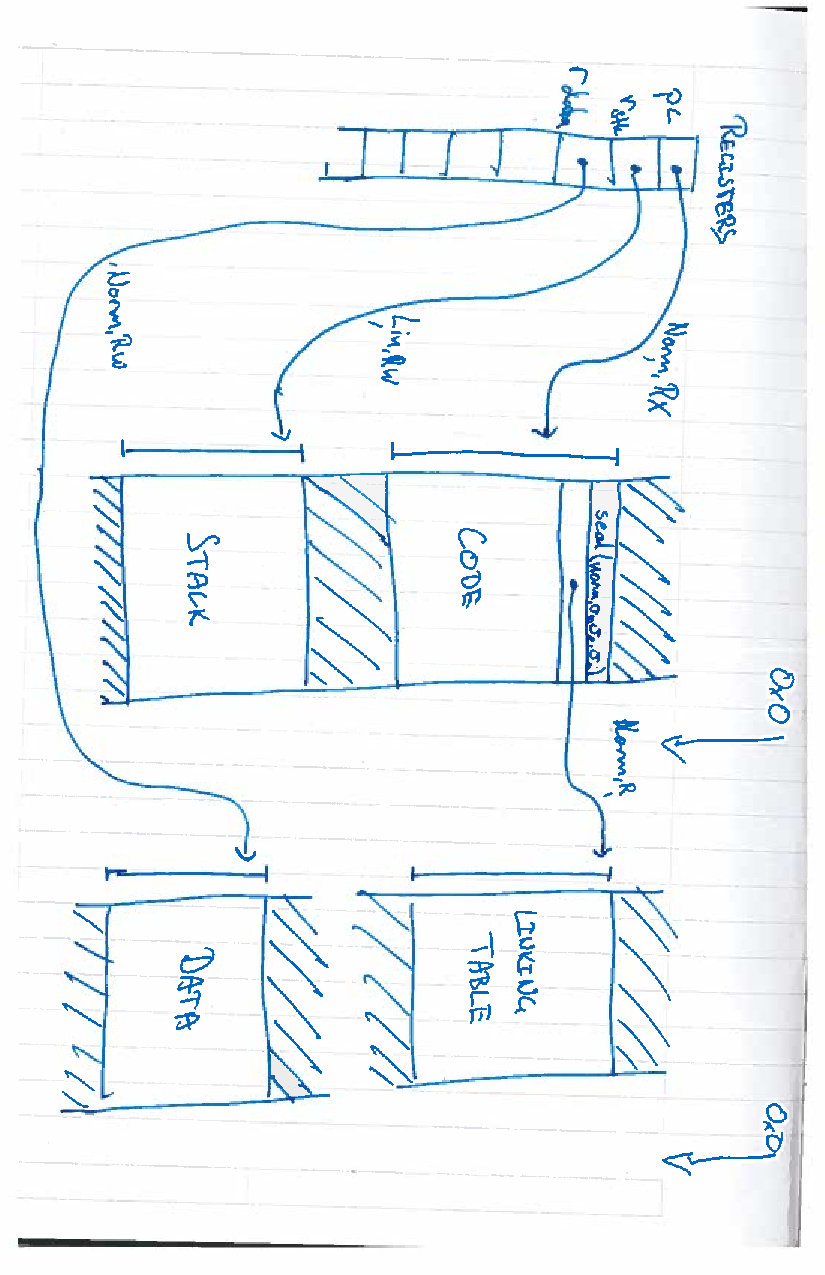
\includegraphics[angle=90,width=\textwidth]{img/linking.pdf}
  \caption{Linking and program layout.}
  \label{fig:trg-prog-link}
\end{figure}

\subsection{Programs and contexts}
\begin{definition}
  \label{def:self-contained}
  \begin{itemize}
  \item We say that a memory segment $\ms$ and a list of words $\bar{w}$
    are self-contained iff
  \[
    \forall w \in \bar{w} \ldotp w \in \Caps \lor w = \stkptr{\_,\_,\_,\_} \Rightarrow \range{w} \subseteq \dom(\ms)
  \]
  and
  \begin{multline*}
    \forall a \in \dom(\ms) \ldotp\\
    (\ms(a) \in Caps \lor \ms(a) = \stkptr{\_,\_,\_,\_}) \Rightarrow \range{\ms(a)} \subseteq \dom{\ms}
  \end{multline*}
  \item We say that a memory segment $\ms$ and a list of capabilities $\bar{c}$ are self contained with slack $\ms_s$ iff
  \[
    \forall c \in \bar{c} \ldotp \range{c} \subseteq \dom{\ms \cup \ms_s}
  \]
  and
  \begin{multline*}
    \forall a \in \dom(\ms) \ldotp\\
    (\ms(a) \in Caps \lor \ms(a) = \stkptr{\_,\_,\_,\_}) \Rightarrow \range{\ms(a)} \subseteq \dom{\ms \cup \ms_s}
  \end{multline*}
\end{itemize}
\end{definition}

\begin{definition}
  \label{def:wxorx}
  ~\\
  A word $w$ is said to respect write-xor-execute iff
  \begin{itemize}
  \item $w \in \ints$
  \item $w = \seal{\_,\_,\_,\_}$
  \item $w = ((\perm,\_),\_,\_,\_) \tand \perm \neq \rwx$
  \item $\seal{\_,\vsc}$ and $\vsc$ respects write-xor-execute
  \item $\src{\stkptr{\perm} \tand \perm \neq \rwx}$
  \item $\src{w = \retptrc(\_,\_)}$
  \item $\src{w = \retptrd(\_,\_)}$
  \end{itemize}
~\\
  A register file $\reg$ is said to respect write-xor-execute with slack $[\bar{r}]$ iff \\
  For all $r \in \RegName$ $\reg(r) \setminus [\bar{r}]$ respects write-xor-execute.
~\\
~\\
  A memory segment $\ms$ is said to respect write-xor-execute iff\\
  For all $\aaddr \in \dom(\ms)$ $\ms(\aaddr)$ respects write-xor-execute
\end{definition}

\begin{definition}
  \label{def:no-stk-ptr}
~\\
  We say that a word $w$ covers no stack pointer iff\\
  \begin{item}
    \item $w \neq ((\perm,\linear),\stkb,\_,\_)$\\
          $\src{w \neq \stkptr{\_,\_,\_,\_}}$
    \item if $w = \sealed{\_,\vsc}$, then $\vsc$ covers no stack pointer.
  \end{item}
~\\
  We say that a memory segment $\ms$ contains no stack pointer iff
  \[
    \forall \aaddr \in \dom(\ms)\ldotp \text{$\ms(\aaddr)$ covers no stack pointer}
  \]
~\\
  We say that a register file $\reg$ contains no stack pointer with slack $[\bar{r}]$ iff
  \[
    \forall r \in \reg \setminus [\bar{r}] \ldotp \text{$\reg(r)$ covers no stack pointer}
  \]
\end{definition}

\begin{definition}
  \label{def:resp-linearity}
~\\
  We say that a memory segment $\ms$ and words $\bar{w}$ respects linearity iff\\
  Let $\var{lc}$ be all the linear capabilities in $\ms$ and $\bar{w}$, i.e.,
  \[
    \var{lc} = \left\{c \middle|
      \begin{array}{l}
        \exists \aaddr \in \dom(\ms) \ldotp c = \ms(\aaddr) = ((\_,\linear),\_,\_,\_) \\
        \exists \aaddr \in \dom(\ms) \ldotp \ms(\aaddr) = \sealed{\_,c} \land c = ((\_,\linear),\_,\_,\_) \\
        \src{\exists \aaddr \in \dom(\ms) \ldotp c = \ms(\aaddr) = \stkptr{\_,\_,\_,\_}} \\
        \src{\exists \aaddr \in \dom(\ms) \ldotp \ms(\aaddr) = \sealed{\_,c} \land c= \stkptr{\_,\_,\_,\_}} \\
      \end{array}
\right\}
  \]
\end{definition}

\subsubsection{Programs}
Here we define what constitutes a program.
\lau{05-10-2017: It seems like both program and context takes care of linking atm.}
\begin{definition}
  \label{def:program}
  \lau{27-09-2017: The ``somehow''s need to be fixed.}
  A program, $\program$ consists of two sealed capabilities, $\vsc_\code = \sealed{c_\code,\sigma}$ and $\vsc_\data = \sealed{c_\data,\sigma}$, and and two memory segments $\ms$ and $\ms_\link$ satisfying
  \begin{itemize}
  \item $c_\code = ((\rx,\lin_\code),\baddr_\code,\eaddr_\code,\aaddr_\code)$ where $\aaddr = \baddr + 2$ and $[\baddr_\code,\eaddr_\code]\subseteq \dom(\ms)$
  \item $c_\data = ((\rw,\lin_\data),\baddr_\data,\eaddr_\data,\baddr_\data)$ where $[\baddr_\data,\eaddr_\data] \subseteq \dom(\ms)$ and $[\baddr_\code,\eaddr_\code] \cap [\baddr_\data,\eaddr_\data] = \emptyset$
  \item $\ms$ and $[c_\code,c_\data]$ are self-contained with $\ms_\link$ as slack.
  \item $\ms$ respects write-xor-execute.
  \item $\ms(\baddr_\code) = \seal{\normal,\sigma_\baddr,\sigma_\eaddr,\sigma_\baddr}$ where these are somehow the sufficient amount of seals.
  \item $\ms(\baddr_\code+1) = ((\ro,\normal),\baddr_\link, \eaddr_\link, \baddr_\link)$ where $\dom(\ms_\link) = [\baddr_\link, \eaddr_\link]$
  \end{itemize}
\end{definition}
\lau{27-09-2017: At the moment, we do not have the proper support to let the code capability be linear (in the sense that you cannot write a sensible program) - maybe we should just require the code capability to be normal.}

\subsubsection{Contexts}
\begin{definition}
  \label{def:context}
  A context, $\context$, is a register file $\reg$, registers $r_1$ and $r_2$, and memory segments $\ms$ and $\ms_\link$ satisfying
  \begin{itemize}
  \item $\reg$ respects write-xor-execute with slack $[r_1,r_2]$.
  \item $\reg(\rstk) = ((\rw,\linear),\stkb,\eaddr,\eaddr)$ where $\stkb \leq \eaddr$\\
        {\sourcecolor{}$\reg(\rstk) = \stkptr{\rw,\stkb,\eaddr,\eaddr}$ where $\stkb \leq \eaddr$}
  \item $\ms \uplus \ms_\link$ respects write-xor-execute
  \item $\ms \uplus \ms_\link$ and $[\reg(\RegName)]$ are self-contained.
  \item $\ms \uplus \ms_\link$ contains no stack pointer.
  \item $\reg$ contains no stack pointer with slack $[r_1,r_2]$.
  \item {\color{red}TODO: No return pointer}
  \end{itemize}
In this definition, the source level specific conditions replace the equivalent target level conditions.
\end{definition}

\subsubsection{Plugging a context}




\section{Compiler}
\label{sec:compiler}
\[
\comp{\cdot} : \src{i}^* \fun \trg{i}^*
\]
\dominique{27-09-2017: Regarding the type signature for $[\cdot]$ above: does this mean that it maps lists of instructions to lists of instructions? Is there another function that compiles a single instruction to a list of instructions?}
\lau{28-09-2017: Yes, that was the thought at the moment, but this may very well change soon. This compiler would then use a compiler that compiles single instructions. That said, this part was added a long time ago and for some reason (some details about the compilation probably did not make sense to me at the moment), I did not complete it. I think the compiler will probably change to be from programs to programs, and a programs is not just going to be a list of instructions.}

\[
  \comp{\scall{r_1}{r_2}} = 
  \begin{array}[t]{l}
    % Make the stack capability into the return capability and seal it:
    %   Push r_data to the stack (should this be made the responsibility of the programmer? If it happens here, then it should probably also be part of the call semantics. Especially, the call semantics should "eat" another piece of memory on the stack to make sure there is no discrepancy.)
    %   Seal the stack capability (with what? where does the seal come from? I think we talked about this, and it is something that should be handled like linking (a fresh seal is available in the beginning of a programs code along with a capability for a linking table)).
    % restrict the stack capability to the unused part (and clear this part (is this really necessary?)).
    % make return capability and ceal it:
    %   Move a copy of pc to a different register.
    %   Adjust the pc copy to point to the return address.
    %   Seal it with the seal.
    % remove all data from temp registers (that is at least the seal).
    % jmpx to r1 and r2
    % restore code:
    %   check the stack end address.
    %   move the stack pointer to the proper register
    %   pop the data capability
  \end{array}
\]

\clearpage

\section{Logical Relation}
\subsection{Worlds}
\lau{30-10-2017: TODO: solve recursiveness in domain equation in the following. }
\lau{02-11-2017: We may need revoked regions again to handle the stack.}
\lau{06-11-2017: If we need to introduce revoked regions like we had for the local capabilities, we may consider the following: For the future world relation require the existence of a bijection from region names to region names. For all regions in the present world the future region is given by the bijection. This would mean that reinstantiation would happen simply by giving a bijection that maps to the new region. In other words, the weird shadowing would not be necessary.
  \begin{mathpar}
    \inferrule{ \dom(W') \supseteq \dom(W) \\ \exists m : \RegionName \fun \RegionName, \text{ $m$ injective} \ldotp \forall r \in \dom(W) \ldotp W'(m(r)) \pubft W(r) }
    { W' \pubft W }
  \end{mathpar}
}
\[
  \World = \RegionName \parfun \Region
\]
where $\RegionName = \nats$.
\[
  \Region = \left\{
  \begin{array}{l}
    \{\spatial \} \times \State \times \Rels \times (\State \fun \World \fun \UPred{\MemSeg^2})\\
    \{\spatialo \} \times \State \times \Rels \times (\State \fun \World \fun \UPred{\MemSeg^2})\\
    \{\pure \} \times \State \times \Rels \times (\State \fun \World \fun \UPred{\MemSeg^2})
  \end{array} \right.
\]
where $\spatial$ and $\spatialo$ are regions governing segments of memory addressed by linear capabilities. $\spatialo$ signifies that this region is addressable. $\spatial$ signifies that the region is not owned and can thus not be addressed. Finally, $\pure$ signifies that the region is only addressed by non-linear capabilities. Notice that no region allows for both linear and non-linear capabilities to address it.
\lau{26-20-2017: We may also want to build the infrastructure for the stack more explicitly into the worlds (but maybe we can handle it in the memory satisfaction).}
\lau{26-20-2017: It is not clear to me what the monotonicity requirements on the memory interpretation functions should be.}
  \[
   \Rels = \{\phi_\pub \times \phi \in \powerset{\State^2}\times \powerset{\State^2} \mid \phi_\pub, \phi \text{ is reflexive and transitive and } \phi_\pub \subseteq \phi \}
  \]


Disjoint union of worlds. Joins together two alike worlds with strictly disjoint ownership over $\spatialo$-regions.
\[
  W_1 \oplus W_2 = W
  \begin{array}[t]{l}
    \text{if $\dom(W) = \dom(W_1) = \dom(W_2) \tand$} \\
    \forall r \in \dom(W) \ldotp W(r) = W_1(r) \oplus W_2(r)
  \end{array}
\]
$\oplus$ is defined as follows
\begin{align*}
  (\pure,\var{sm}) \oplus (\pure,\var{sm}) =  & \; (\pure,\var{sm}) \\
  (\spatialo,\var{sm}) \oplus (\spatial,\var{sm}) = & \; (\spatial,\var{sm}) \oplus (\spatialo,\var{sm})\\
                                           =  & \; (\spatialo,\var{sm}) \\
  (\spatial,\var{sm}) \oplus (\spatial,\var{sm}) =  & \; (\spatial,\var{sm}) \\
\end{align*}
and for all other cases $\oplus$ is undefined. Specifically, $\oplus$ is not defined when both sides are a $\spatialo$-region. It is further not defined if the two sides do not agree on region type and state machine. Here $\var{sm}$ is the state machine of the region.

\subsection{Future world}


\subsection{Memory satisfaction}
\[
  \memSat{\ms_S,\ms_\stk,\stk,\ms_T}{W} \text{ iff } 
  \left\{
    \begin{array}{l}
      \exists R_\ms : \dom(W) \fun \MemSeg^2 \ldotp \\
      \quad \ms_T = \biguplus_{r \in \dom(W)} \pi_2(R_\ms(r)) \wedge \\
      \quad \stk = (\_,\ms_{\stk,0}) :: \dots :: (\_,\ms_{\stk,m}) \wedge \\
      \quad \exists r_0 , \dots, r_m, r_{m+1} \ldotp \pi_1(R_\ms(r_0,\dots,r_m)) = \ms_{\stk,0},\dots , \ms_{\stk,m} \wedge \\
      \qquad \pi_1(R_\ms(r_{m+1})) = \ms_\stk \wedge \\
      \qquad \ms_S \uplus \ms_\stk \uplus \ms_{\stk,0} \uplus \dots \ms_{\stk,m} = \biguplus_{r \in \dom(W)} \pi_1(R_\ms(r)) \wedge \\
      \qquad \exists R_w : \dom(W) \fun \World \ldotp\\
      \quad \qquad W = \bigoplus_{r \in \dom(W)} R_w(r) \wedge \\
      \quad \qquad \forall r \in \dom(W) , n' < n \ldotp \\
      \qquad \qquad \npair[n']{R_\ms(r)} \in W(r).H \; (W(r).s) \; (\xi^{-1} (R_w (r))) 
    \end{array}
  \right.
\]
In the definition of memory satisfaction, $R_\ms$ acts as a partitioning in the two related memories. As the source language is a special interpretation of the target language, part of the target memory needs to relate to the stack in the source language. We also need to split up the world which is done by $R_W$.We split up the world in order to make sure that the linearity constraints imposed by the world are satisfied.
\lau{30-10-2017: It is not clear to me whether this definition should also talk about $\opc$.}

\subsection{Relation}
\lau{19-10-2017: Rest of source configuration needs to come from somewhere in $\lre$.}
\lau{19-10-2017: Maybe linearity should be taken care of in just one place (instead of in $\lrr$ relation and mem satisfaction). That is, add a predicate that checks whether the configuration satisfies linearity (such a condition may be to syntactic to work?).}
In the following definitions, \src{blue} is used to indicate values related to the source machine. This is unlike previous definitions, where \src{blue} is used  indicate source language specific parts of definitions.
\[
  \lre(W) = \left\{ \npair{\stpair[.]{v_{c,S},v_{d,S}}{v_{c,T},v_{d,T}}} \middle| 
    \begin{array}{l}
      \forall n' \leq n, \src{k_{d,S}}, \src{k_{c,S}}, k_{d,T}, k_{c,T}, \src{\reg_S}, \reg_T, \src{\ms_S}, \ms_T, \src{\ms_\stk}, \src{\stk} \ldotp\\
      \quad \forall W_\lrk, W_\lrr, W_\lrm \ldotp \\
      \qquad\npair[n']{\stpair[.]{v_{c,S},v_{d,S}}{v_{c,T},v_{d,T}}} \in \lrp(W) \wedge \\
      \qquad\npair[n']{\stpair[.]{k_{d,S},k_{c,S}}{k_{d,T},k_{c,T}}} \in \lrk(W_\lrk) \wedge \\
      \qquad\npair[n']{\stpair{\reg}{\reg}} \in \lrr(W_\lrr) \wedge\\
      \qquad\memSat[n']{\stpair[.]{\ms_S,\stk,\ms_\stk}{\ms_T}}{W_\lrm} \\
      \qquad\Rightarrow\\
      \qquad\npair[n']{\left(\array{l}\src{(\ms_S,\reg_S\updReg{\pcreg,\rdata,\rretc,\rretd}{v_{c,S},v_{d,S},k_{c,S},k_{d,S}},\stk, \ms_\stk)},\\
                                          (\ms_T,\reg_T\updReg{\pcreg,\rdata,\rretc,\rretd}{v_{c,T},v_{d
,T},k_{c,T},k_{d,T}})\endarray\right)}
      \in \lro(W\oplus W_\lrk \oplus W_\lrr \oplus W_\lrm)
    \end{array}
    \right\}
\]
\lau{24-10-2017: Dominique, I do not see how the splitting of worlds is going to work out. I can see how it will enforce linearity, but is you give a "spatial" region (the kind of region that is only allowed to go to one part of a split) to the $\lrr$-relation, then the memory satisfaction does not have it, and it cannot find a memory segment for this part. In other words, the memory satisfaction will not be able to find a concrete memory segment for segments governed by a linear capability in the register file. Maybe the memory satisfaction should have all of the parts, so it can represent them (but also limit what linear capabilities can be used).}

\[
  \lro(W) = \left\{ \npair{\left(\array{l}\src{(\ms_S,\reg_S,\stk_S,\ms_{\stk,S})},\\(\ms_T,\reg_T)\endarray\right)} \middle|
    \begin{array}{l}
      \forall i \leq n \ldotp \\
      \quad \src{(\ms_S,\reg_S,\stk_S,\ms_{\stk,S})} \term[i] \Rightarrow (\ms_T,\reg_T) \term\\
      \quad \tand\\
      \quad (\ms_T,\reg_T) \term[i] \Rightarrow \src{(\ms_S,\reg_S,\stk_S,\ms_{\stk,S})} \term
    \end{array}
\right\}
\]


\lau{03-11-2017: TODO take a look at linearity of this definition - in particular the recovered pc and stack pointer.}
\[
  \lrk(W) = \left\{ \npair{\left(\array{l}\src{\retptrd(\sigma,(\aaddr_d,\eaddr_d))},\\\src{\retptrc(\sigma,(\perm,\lin,\baddr_c,\eaddr_c,\aaddr_c))},\\k_{d,T},k_{c,T}\endarray\right)} \middle|
    \begin{array}{l}
      k_{d,T} = \sealed{\sigma,c_d} \wedge\\
      k_{c,T} = \sealed{\sigma,c_c} \wedge\\
      c_c = ((\perm,\lin),\baddr_c,\eaddr_c,\aaddr_c) \wedge\\
      c_d = ((\rw,\linear),\aaddr_d,\eaddr_d,\aaddr_d-1) \wedge\\
      \forall n' \leq n, W' \pubft W \ldotp \\
      \quad \forall, W_\lrr, W_\lrm \ldotp  \\
      \qquad\opc = c_c \wedge\\
      \qquad\dom(\ms_{\stk,f}) = [\aaddr_d,\eaddr_d] \wedge\\
      \qquad\npair[n']{\src{\retptrd(\sigma,\_)},\src{\retptrc(\sigma,\_)},k_{d,T},k_{c,T}} \in \lrp(W') \wedge \\
      \qquad\npair[n']{\stpair{\reg}{\reg}} \in \lrr(W_\lrr) \wedge\\
      \qquad\memSat[n']{\stpair[.]{\ms_S,\stk::(\opc,\ms_{\stk,f}),\ms_\stk}{\ms_T}}{W_\lrm} \wedge \\
      \qquad\src{reg_S}(\rstk) = \src{\stkptr{\rw,\baddr_\stk,\eaddr_\stk,\_}} \wedge \\
      \qquad\eaddr_\stk = \aaddr_d-1\\
      \qquad\Rightarrow\\
      \qquad\npair[n']{\left(\array{l}\src{\left(\arraycolsep=0pt\array{l}\ms_S,\reg_S\updReg{\pcreg,\rstk}{\opc,\stkptr{\rw,\baddr_\stk,\eaddr_d,\aaddr_d}},\\\stk, \ms_\stk \uplus \ms_{\stk,f}\endarray\right)},\\
                                          (\ms_T,\reg_T\updReg{\pcreg,\rstk}{\opc,((\rw,\lin),\baddr_\stk,\eaddr_d,\aaddr_d)})\endarray\right)}
      \in \lro(W' \oplus W_\lrr \oplus W_\lrm)
    \end{array}
  \right\}
\]

\[
  \lrp(W) = \left\{
    \npair{\stpair{v}{v}} \middle| \text{make sure linearity constraint satisfied}\dots 
  \right\}
\]


\[
  \lrr(W) = \left\{ \npair{\stpair{\reg}{\reg}} \middle|
    \begin{array}{l}
      \exists S : \RegName \fun \World \ldotp \\
      \quad S \text{ is a separation of $W$} \tand\\
      \quad \forall r \in \RegName \setminus \{\pcreg, \rretd,\rretc,\rdata \}\ldotp\\
      \qquad\npair{\stpair[.]{\src{\reg_S(r)}}{\reg_T(r)}} \in \lrv(S(r))
    \end{array}
            \right\}
\]
Where $S\text{ is a separation of $W$}$ means that no two partition share the same ``spatial'' region (whatever that is).

\[
  \lrv(W) =
  \begin{array}[t]{l}
    \left\{ \npair{\stpair[.]{i}{i}} \;\middle|\; i \in \ints \right\}\cup \\
    \left\{ \npair{\left(\arraycolsep=0pt\array{l}\src{\retptrc(\sigma,\_)},\\\sealed{\sigma,\vsc_C}\endarray\right)} \;\middle| \;
    \begin{array}{l}
    \forall n'<n, W' \pubft W, W_\lrv \npair[n']{\stpair[.]{\retptrd(\sigma,\_)}{\sealed{\sigma,\vsc_D}}} \in \lrv(W_\lrv) \ldotp\\
      \npair[n']{\retptrc(\sigma,\_),\retptrd(\sigma,\_),\sealed{\sigma,\vsc_C},\sealed{\sigma,\vsc_D}} \in \lrk(W' \oplus W_\lrv)
    \end{array}
    \right\}\cup\\
    \left\{ \npair{\left(\arraycolsep=0pt\array{l}\src{\retptrd(\sigma,\_)},\\\sealed{\sigma,\vsc_D}\endarray\right)} \;\middle| \;
    \begin{array}{l}
    \forall n'<n, W' \pubft W, W_\lrv \npair[n']{\stpair[.]{\retptrc(\sigma,\_)}{\sealed{\sigma,\vsc_C}}} \in \lrv(W_\lrv) \ldotp\\
      \npair[n']{\src{\retptrc(\sigma,\_)},\src{\retptrd(\sigma,\_)},\sealed{\sigma,\vsc_C},\sealed{\sigma,\vsc_D}} \in \lrk(W' \oplus W_\lrv)
    \end{array}
    \right\}\cup \\
    \left\{ \npair{\left(\arraycolsep=0pt\array{l}\src{\sealed{\sigma,\vsc_S}},\\ \sealed{\sigma,\vsc_T} \endarray\right)} \;\middle| \;
    \begin{array}{l}
      
    \end{array}
    \right\}\cup\\
    \left\{ \npair{\left(\arraycolsep=0pt\array{l} \src{\seal{\sigma,\sigma_\baddr,\sigma_\eaddr}},\\ \seal{\sigma,\sigma_\baddr,\sigma_\eaddr} \endarray \right)} \;\middle|\;
    \right\} \cup \\
    \left\{ \npair{\left(\arraycolsep=0pt\array{l} \src{\stkptr{\perm,\baddr,\eaddr,\aaddr}},\\ ((\perm,\linear),\baddr,\eaddr,\aaddr) \endarray \right)} \;\middle|\;
    \right\} \cup \\
    \left\{ \npair{\left(\arraycolsep=0pt\array{l} \src{((\perm,\lin),\baddr,\eaddr,\aaddr)},\\ ((\perm,\lin),\baddr,\eaddr,\aaddr) \endarray \right)} \;\middle|\; 
    \begin{array}{r l l }
      \perm \in \readAllowed{} &\Rightarrow& \npair{\baddr,\eaddr} \in \readCond{\lin,W}\\
      \perm \in \writeAllowed{} &\Rightarrow& \npair{\baddr,\eaddr} \in \writeCond{\lin,W}\\
      \perm = \rwx &\Rightarrow& \npair{\{\rwx,\rx\},\baddr,\eaddr} \in \execCond{\lin,W}\\
      \perm = \rx &\Rightarrow& \npair{\{\rx\},\baddr,\eaddr} \in \execCond{\lin,W}
    \end{array}

    \right\}
  \end{array}
\]

\subsection{Permission based conditions}
\[
  \addressable{\lin,W} =
  \begin{cases}
    \{ r \mid W(r) = (\normal,\_) \} & \text{if $\lin = \normal$} \\
    \{ r \mid W(r) = (\spatialo,\_) \}  & \text{otherwise (i.e. $\lin = \linear$)} \\
  \end{cases}
\]

\[
  \readCond{\lin,W} = \left\{ \npair{\baddr,\eaddr}) \middle| 
    \begin{array}{l}
      \exists r \in \addressable{\lin, W} \ldotp \\
      \quad \exists [\baddr',\eaddr'] \supseteq [\baddr,\eaddr] \ldotp \\
      \qquad W(r) \nsubeq \iota_{[\baddr',\eaddr']}
    \end{array}
  \right\}
\]
where $\iota_A$ is a standard region defined in Section~\ref{sec:standard-regions}.

\begin{definition}
  \label{def:address-stratified}
  We say that a region $\iota = (\_,\_,\_,\_,H)$ is address stratified iff
  \[
    \begin{array}{l}
      \forall n, \src{\ms_S},\ms_T,\src{\ms_S'},\ms_T',s,\hat{W}\ldotp \\
      \quad \npair{\stpair{\ms}{\ms}}, \npair{\stpair[.]{\ms_S'}{\ms_T'}} \in H \; s \; \hat{W} \wedge \\
      \quad \dom(\src{\ms_S}) = \dom(\ms_T) = \dom(\src{\ms_S'}) = \dom(\ms_T') \\
      \quad \Rightarrow \\
      \qquad \forall \aaddr \in \dom(\ms_S) \ldotp \npair{(\src{\ms_S}\update{\aaddr}{\src{\ms_S'}(\aaddr)},\ms_T\update{\aaddr}{\ms_T'(\aaddr)})} \in H \; s \; \hat{W}
    \end{array}
  \]
\end{definition}

\[
  \writeCond{\lin,W} = \left\{ \npair{\baddr,\eaddr}) \middle| 
    \begin{array}{l}
      \exists r \in \addressable{\lin, W} \ldotp \\
      \quad \exists [\baddr',\eaddr'] \supseteq [\baddr,\eaddr] \ldotp \\
      \qquad W(r) \nsupeq[n-1] \iota_{[\baddr',\eaddr']} \wedge \\
      \qquad W(r) \text{ is address-stratified}
    \end{array}
  \right\}
\]
where $\iota_A$ is a standard region defined in Section~\ref{sec:standard-regions}.

\[
  \execCond{\lin,W} = \left\{ \npair{S_\perm,\baddr,\eaddr} \middle|
    \begin{array}{l}
      \forall n' < n, W' \privft W, \perm \in S_\perm, \aaddr \in [\baddr,\eaddr] \ldotp\\
      \quad \forall W'', c_{d,S},c_{d,T} \ldotp \npair[n']{(c_{d,S},c_{d,T})} \in \lrv(W'') \wedge \\
      \qquad \npair[n']{((\perm,lin),\baddr,\eaddr,\aaddr),c_{d,S},((\perm,lin),\baddr,\eaddr,\aaddr),c_{d,T}} \in \lrp(W' \oplus W'') \Rightarrow \\
      \quad \qquad \npair[n']{((\perm,lin),\baddr,\eaddr,\aaddr),c_{d,S},((\perm,lin),\baddr,\eaddr,\aaddr),c_{d,T}} \in \lre(W' \oplus W'')
    \end{array}
    \right\}
\]


\subsection{Standard regions}
\label{sec:standard-regions}
Standard region:
\[
  \iota_A \defeq (\normal,*,=,=,H_A)
\]
\lau{02-11-2017: I am not sure whether it should be a $\normal$ region. In previous work $\nsubeq$ ignored the ``view'' which it may also do here, and then then it does not matter which one it is.}
where $H_A$ is defined as follows:
\[
  H_A \; s \; \hat{W} \defeq \left\{ \npair{\ms_S,\ms_T} \middle|
    \begin{array}{l}
      \dom(\ms_S) = \dom(\ms_T) = A \wedge \\
      \forall \aaddr \in A \ldotp \npair[n-1]{(\ms_S(\aaddr),\ms_T(\aaddr))} \in \lrv(\xi(\hat{W}))
    \end{array}
  \right\}
\]
\lau{01-11-2017: TODO look into what kind of world separation should happen here.}

\section{Full Abstraction}
\begin{definition}
  \label{def:points-to-instr}
  A configuration $(\ms,\reg)$ {\sourcecolor or $(\ms,\reg,\_,\_)$} is said to point instruction $i$ in $A$ iff
  \[
    \reg(\pcreg) = ((\_,\_),\_,\_,\aaddr) \tand \aaddr \in A
  \]
and
\[
  \decInstr{\ms(\aaddr)} = i
\]
\end{definition}

We want to make a conditional full-abstraction statement. The condition should express two things (1) the compilation so far has been reasonable, so we do not have to setup protection against things any reasonable compiler wouldn't do. (2) the compilation so far has taken care of certain checks that we do not have information to place correctly at this point of the compilation
\begin{definition}
  \label{def:check-stack-addr-before-call}
  A configuration $\src{\Phi}$ is said to have reasonable calls in $A$ for $n$ steps iff\\
  for all $i \leq n$ if
  \[
    \src{\Phi} \nstep[i] \src{\Phi'}
  \]
  and $\src{\Phi'}$ points to $\src{\scall{r_1}{r_2}}$ in $A$ for some $\src{r_1}$ and $\src{r_2'}$ and there exists no $j<i$ s.t.
  \[
    \src{\Phi} \nstep[j] \src{\Phi''}
  \]
  where $\src{\Phi''}$ points to $\src{\scall{r_1'}{r_2'}}$ in $A$ for some $\src{r_1'}$ and $\src{r_2'}$,
  then
  \[
    \src{\Phi}(\src{r_\stk}) = \src{\stkptr{\_,\stkb,\_,\_}}
  \]
  and $\src{\Phi'}$ has reasonable calls in $A$ for $n-i$ step.
\end{definition}

\begin{definition}
  A program $\program$ with memory segment $\ms_\program$ is said to be reasonably compiled if for all $n$ and all contexts $\context$ the configuration $\plug{\context}{\program}$ satisfies:
  \begin{itemize}
  \item $\plug{\context}{\program}$ has reasonable calls in $\dom(\ms_\program)$ for $n$ steps.
  \end{itemize}
\end{definition}

\begin{theorem}
  \label{thm:full-abstraction}
  For programs $\program_1$ and $\program_2$ that are reasonably compiled compiled, we have
  \begin{gather*}
    \src{\program_1} \sconeq \src{\program_2}\\
    \Updownarrow\\
    \comp{\src{\program_1}} \tconeq \comp{\src{\program_2}}
  \end{gather*}
\end{theorem}

\clearpage
\section{Examples}
\subsection{Capability Opacity}
\label{subsec:capability-opacity}

\dominique{27-09-2017: Is this example still relevant? Isn't it solved differently by the variable-length-instructions idea?}
\lau{28-09-2017: It seems to me that this is indeed solved by the variable length instructions. That said, I would like to keep it around (maybe change it so it becomes an argument for variable length instructions).}
This example was introduced when we envisioned a capability machine with $\spush{}$, $\spop{}$, $\ssload{}{}$, $\scall{}{}$ and $\sreturn$ instructions. The below example is a motivation for having variable length instructions in the source language because if we have enough memory to ``do the same'' in the target language as in the source language, then the below example does not work.

The following pseudo program demonstrates the need of opaque capabilities. If we assume a system with no opaque capabilities, then the following programs break compiler correctness
\begin{lstlisting}[basicstyle=\sourcecolor{}\ttfamily] 
p1 ::= if r1 is length 2 then
         call r1 with the following callback in r5:
           {put $\textit{\texttt{diverging}}$ closure in r2;
            return};
         halt
       else diverge

p2 ::= if r1 is length 2 then
         call r1 with the following callback in r5:
           {put $\textit{\texttt{terminating}}$ closure in r2;
            return};
         halt
       else diverge
\end{lstlisting}
The diverging closure could just contain $\sjmp{\pcreg}$, which diverges. The terminating closure could just be $\sreturn$.

The context with $r1$ as an executable capability pointing to:
\begin{lstlisting}[basicstyle=\sourcecolor{}\ttfamily] 
$\scall{r5}{0}$
$\sjmp{r5}$
\end{lstlisting}
\footnote{At this time $\scall{}{}$ did argument spilling and it only takes one argument because we were considering enter capabilities.}distinguishes the two contexts, but two instructions are not enough to do the same at the target level. We would not have enough instructions to set up a proper return pointer for the compiled return to use.

\clearpage
\section{Back translation}
The back translation is an embedding of source language into .

\section{Notes}
\subsection{Leuven stay conclusions}
\begin{enumerate}
\item Enter capabilities replaces by sealed code/data pairs \label{item:first-point}
  \begin{itemize}
  \item To allow us to forbid dynamic code generation
  \end{itemize}
\item Conditional full-abstraction
  \begin{itemize}
  \item No undefined behaviour by \emph{trusted code} in any context implies full-abstraction. (Blame idea: undefined as undef of current pc, so current pc can be checked for whether it was the trusted code).
  \item Avoids dynamic checks to protect trusted code against itself.
  \item Possible due to point \ref{item:first-point}.
  \end{itemize}
\item replace push/pull/call/ret/sload by symbolic return pointer (pair) and stack pointer.
  \begin{itemize}
  \item Allows back translation to be embedding into source language.
    \begin{itemize}
    \item Interpreter for back translation is not able to accurately replicate code length.
    \end{itemize}
  \end{itemize}
\item Worlds similar to CSF paper, but invariants on seals as well.
  \begin{itemize}
  \item Invariants says what can be sealed with a certain seals.
  \end{itemize}
\item Linker: resolves symbols
  \begin{itemize}
  \item Export refs (Question: do we allow other things than sealed code/data pairs to be exported?)
  \item Import refs
  \item Fresh seal requirement
  \end{itemize}
\item Components are memory segments and symbols.
\item Variable instruction length in the source to avoid leaking information through code size that cannot be matched after compilation (breaks compiler correctness, see example in subsection~\ref{subsec:capability-opacity}).
  \begin{itemize}
  \item Notice x86 allows instructions of up to infinite length, so this is not weird.
  \end{itemize}
\item Have opaque capabilities.
  \begin{itemize}
  \item Without opaque capabilities, stack consumption could be inferred through stack pointer index etc.
  \end{itemize}
\item Considered PORs for transition systems to: ($a \rightarrow b \Rightarrow a \rightarrow a \text{ and } b \rightarrow b$)
  \dominique{27-09-2017: I don't remember what we meant with PORs, but perhaps quasi-reflexive partial orders.  Not sure what the point of this was again... }
  \lau{28-09-2017: I think the next three points is the answer. We basically wanted a formalism in which we could design one region that would govern the stack. I do not remember why it was made possible with PORs.}
  \begin{itemize}
  \item Define one region that governs the stack
  \item Make the regions more general
  \item For now, we have not done this: instead we stick with the transition systems we have and have two regions governing the stack reflecting the CSF work.
  \end{itemize}
\end{enumerate}

\subsection{Some explanation}
\subsubsection{The source language}
The whole idea of this paper is to show that we enforce well-bracketed control flow correctly by taking a source language with a native stack and native call and return instructions and well-bracketedness enforced by the operational semantics.
We then prove that we can compile this source language to a regular assembly target language (without a native stack) in a fully abstract way using our stack and return pointer discipline.
So the design goals for our source language were precisely these: it should be an intermediate language that stays as close as possible to our target language, can be fully abstractly compiled to the target and feature a native well-behaved stack.
This source language can then be used as the second-to-last language in the compilation chain of a fully abstract compiler.
By compiling in a fully abstract way to our source language and then composing with our compiler, fully abstract compilation to our target language follows easily.

These design goals drove us to the current definition of our source language and some special design choices.
Particularly, contrary to what one might expect in a language with a native stack, we do not use call/return and push/pop instructions.
The reason is that we are working in a language where the length of code blocks can be observable.
Imagine two trusted blocks of code that looks as follows:
\begin{lstlisting}[basicstyle=\sourcecolor{}\ttfamily] 
p1:       <assert that r1 contains an executable capability to a block of 
           instr_length (push) + instr_length(jmp)> 
          <load return capability to p1-ret1 in r2>
          <load value 0 in r3>
          <jump to r1>
p1-ret1:  <assert that 0 is loaded in the next free stack position>
          <repeat the above with value 1 in r3>
          ...
p1-ret2:  <assert that 1 is loaded in the next free stack position>
          <repeat the above with value 2 in r3>
          ...
p1-ret3:  <assert that 2 is loaded in the next free stack position>
          halt

p2:       <assert that r1 contains an executable capability to a block of 
           instr_length (push) + instr_length(jmp)>
          <load return capability to p2-ret1 in r2>
          <load value 1 in r3>
          <jump to r1>
p2-ret1:  <assert that 1 is loaded in the next free stack position>
          <repeat the above with value 2 in r3>
          ...
p2-ret2:  <assert that 2 is loaded in the next free stack position>
          halt
\end{lstlisting}

p1 and p2 each accept an (unprotected) closure from the context whose length is restricted.
Together with the checks performed by p1 and p2, there is only one possible implementation of the closure that will not fail, namely
\begin{lstlisting}[basicstyle=\sourcecolor{}\ttfamily] 
closure: push r3
         jmp r2
\end{lstlisting}

However, this is no longer true in the target language.
Assume that $\mathtt{push r3}$ is implemented as a store to $\rstk$ followed by an increment of $\rstk$.
The adversary can now construct a closure that does not use the standard implementation of push, but instead does this:
\begin{lstlisting}[basicstyle=\targetcolor{}\ttfamily] 
evil-closure: jnz r3 r2
              store $\rstk$ r3
              jmp r2
\end{lstlisting}
If we now assume that the instructions in evil-closure (jnz+store+jmp) are the same length as the original closure(store+increment+jmp), then the adversary can now construct a closure that discriminates $\mathtt{p1}$ and $\mathtt{p2}$ above.
The essential point here is that an assumption in the source language that relies on facts about instruction length (``a closure restricted to the instruction-size of push+ret that modifies the stack and returns can only be implemented in one way'') is no longer valid, because there are now more low-level ways of interacting with the stack.

To remedy this, we decided to modify our source language to use a different way of interacting with the stack.
This alternative approach stays even closer to the target language.
The problem is not actually that we shouldn't offer push/pop and call/return instructions, but rather that our language should also offer an equivalent for the more low-level interactions with the stack that are possible in the target language.
As such, we introduce special token values that play the role of the stack pointer/return pointer and we allow all interactions with them that are possible using instructions like \sstore{}{}, \smove{}{} etc.
Specifically, as shown in \cref{sec:domains}, there are new token capabilities $\stkptr{\permbnf,\basebnf,\aendbnf,\addrbnf}$, $\retptrd$ and $\retptrc$ which represent a copy of the stack pointer, and the code and data parts of the sealed return closure.
Rather than invoking \spush{} or \spop{}, one can store into the $\stkptr{}$ and modify its current address and as we can see in \cref{sec:source-language}, this has the semantic effect that one would expect.
Similarly, rather than invoking \sreturn{}, one would ccall the $\retptrd$ and $\retptrc$ sealed code/data pair.

We do not offer primitive \sreturn{}, \spush{} and \spop{} instructions, even though there is nothing keeping us from doing that, either as an additional primitive instruction or as a macro on top of the primitive token values mentioned above.
We do offer a primitive \scall{}{} instruction, and it offers the only way to create a new stack frame.
It is the only instruction that does not have a target language counterpart.
However, there is a counterpart to \sxjmp{}{}, the instruction that would be used for jumping in the code that \scall{}{} compiles to.
We will discuss later that this means that if we back translate an adversary piece of code (in the full abstraction proof), then it will be back translated (under our trivial back-translation) to equivalent code that \emph{never} does an actual call, but always just jumps to where it wants to go.
In other words, the back-translated code never uses call to protect its own stack frame from the code that it passes control to.
This means that the back-translated code is quite insecure, but we don't need it to be: it just needs to be behaviorally equivalent to the target language code that it represents.

% Finally, rather than invoking call, \dominique{7-9-2017: err, what's the reason we don't follow the same pattern for call?}.
% \lau{07-09-2017: One would use $\scall{}{}$ with a pair of sealed capabilities to securely jump to this pair - that is to have this pair executed in a new stack frame. The return would happen just by using $\sxjmp{}{}$ with the $\retptrd$ and $\retptrc$. However, this would work with the local capabilities as the real implementation of $\retptrd$ would be a sealed version of the entire stack pointer. In other words, upon jumping back no extra work would have to be done. Now, however, the old stack pointer should be spliced (using the new $\ssplice{}{}$ instruction) with the stack pointer we sent away in order to regain the old stack pointer. In other words, we need something to recognise when a return happens.}
% \lau{07-09-2017: On second thought, when compiled all the code necessary for the call will be generated based on the $\scall{}{}$ instruction. The real implementation of the $\retptrc$ will simply point to a piece of clean up code that splices together the old/private stack pointer with the one we got from the untrusted party. This may, however, give some issues when we want to reason about it because there will be a disconnect between where the clean up job is done in the operational semantics of the source language (namely as part of the $\sxjmp{}{}$), but in a translated program, the code that does the clean up origins with the $\scall{}{}$ instruction. }

Note that the token values representing the stack and return pointer in our source language are essentially just a weird alternative syntax for something we would otherwise write using call/return and push/pop.
However, it does remove the problem described above of relying on facts that follow from code length, because we can now write exactly the same code in source and target and it will do exactly the same thing if it is well-behaved.
The code would look exactly the same in source and target, it would just be working with token values in the source versus real stack and return pointers in the target.
That the problem is really gone should follow from being able to write a full-abstraction proof.
However, our approach should also simplify that proof.
The reason is that back-translating should become essentially trivial: rather than performing some form of emulation or a real back-translation (which would inevitably make code size larger), it should be sufficient to just use unmodified target instructions as source instructions that will just be working with different types of values.


\subsubsection{Conditional full abstraction}
\label{sec:conditional-full-abstraction}

Another novelty in this work is the fact that we do not want to prove general full abstraction (i.e. two source programs are behaviorally equivalent if and only if they are compiled to behaviorally equivalent target programs).
The reason is that we only want to prove a result about programs that respect the calling convention, i.e.\ that do not do anything stupid.
For example, in the old setup with global/local capabilities, when trusted code performs an \scall{}{}, it should make sure that it does not store a copy of its stack pointer in a place that is accessible to the callee (e.g.\ in a register or in the callee's part of the stack).
Such sanity conditions are necessary (we cannot guarantee anything for code that does such stupid things) but we do not want to spend computation time on checking them.
Instead, we expect a reasonable compiler to guarantee in some way that its generated code never does such stupid things and then our guarantees should apply.

Note that in the new setup with linear capabilities instead of local/global ones, there seems to be less opportunity for the trusted code to do stupid things, so it may be that we no longer need these sanity conditions, but this is not clear yet.

Assuming that we need sanity conditions on the source code, the question is how we formulate them in our full abstraction.
Our idea is to formulate a notion of conditional full abstraction: ``if source programs t1 and t2 never perform stupid things under any possible source interaction, then they are source-equivalent iff their compilations are target-equivalent.''.
However, the question remains how we formalise the condition ``if source programs t1 and t2 never perform stupid things under any possible source interaction''.

Two possible approaches:
\begin{itemize}
\item \emph{Blame}: the idea here would be that we introduce a notion of ``undefined behavior'' in the operational semantics.
  ``Doing stupid things'' like leaving copies of the stack pointer around on a call, would cause the system to enter an undefined state.
  We would then like to express the above mentioned sanity condition as ``t1 and t2 never evaluate to undefined when plugged into an arbitrary program context''.
  However, that doesn't work, because it does not discriminate between undefined behavior caused by t1 or t2 (on the one hand) and the program context (on the other hand).
  To remedy this, we intended to use a notion of blame assignment: the undefined state would contain the address of the pc that was active at the moment it went wrong.
  We would then express the above mentioned sanity condition as ``t1 and t2 never evaluate to undefined(pc) where pc is within the trusted code's assigned code memory when plugged into an arbitrary program context''.

  The problem with this approach is that it does not combine well with dynamically generated code (solution: exclude code-generation?) and that it adds a lot of complexity.

\item \emph{A logical relation}: An alternative approach (suggested by Lars to Lau) might be to define a logical relation to express the sanity condition ``t1 and t2 never evaluate to undefined when plugged into an arbitrary program context''.
  This remains to be thought through in more detail, but it might be simpler and/or be easier to combine with dynamic code generation.
\end{itemize}

\subsection{Linear Capabilities}
\label{sec:linear-cap}
The idea with linear capabilities is to limit aliasing of a capability. We specifically wanted a linear capability for the stack pointer, to not have to erase large pieces of memory, which we have to when we use local capabilities. With linear capabilities, we would just need to find the one linear capability to be sure we have the only capability under our control.

There are multiple ways that linear capabilities could work (we choose the third one):
\begin{enumerate}
\item A linear capability comes with a system wide guarantee that no \emph{linear} alias exists for this capability (or any part of the memory it has authority over). In other words, the linear capability is the only \emph{linear} capability for this piece of memory.  However, non-linear aliases may exist.

In order for this to work, the memory must initially be partitioned into two parts. One controlled by a non-linear capability and one controlled by a linear capability. The semantics of the machine would now have to make sure that the linear capability is never aliased. For instance, moving a linear capability from one register would cause the source register to be cleared (similar to destructive reads in the ownership types literature). 

In this scheme, it would be okay to permit linear capabilities to become non-linear (which would consume the linear capability). The reasoning would be that it is okay to remove the aliasing restriction and thus make the part of memory with the no-aliasing guarantee smaller. If some program depends on a certain capability received from an adversary to be linear, then they would simple have to check whether it is in fact linear. As the linear capability is consumed when making it non-linear, it would have no way to regain the linear capability.

\item A linear capability can be created from a non-linear capability. The linear capability has no guarantee that it is not aliased, but no aliases can be made from the linear capability. The linear capability can now be passed to an adversary and if the adversary gives back the linear capability when they return, then we know that they have no alias for it (provided we did not give them one and they did not have one in the first place), because the linear capability does not permit them to create an alias.

In this scheme, the system would initially have one non-linear capability for all of the memory. The linear capabilities would then be generated as they are needed.
\item A linear capability is ``born'' with the guarantee that it is not aliased, either by linear or non-linear capabilities. This guarantee is maintained by the semantics. Linear capabilities cannot be converted to another kind of capability (in other words, this is option one but where linear capabilities cannot be made non-linear).

Note that in this scheme, it would be good if malloc provided a way to initially obtain a linear capability in this model.
Otherwise, there would never be any linear capabilities other than stack pointers, which seems a waste.
\end{enumerate}
Notice that the two first schemes are incompatible as they would undermine each other.

We chose to use the second scheme for the following reasons:
\begin{itemize}
\item While the stack pointer was the motivation for the linear capabilities, we believe they can also be used for other things such as return pointers. When used for return pointers, we know that the return pointer used to return to us was the only one available. However, if we used the first scheme, then all of the code would have to be in the linear part of memory. This would be undesirable if we want to provide several entities access to the same program. 
\end{itemize}
We later abandoned the second option for the following reason:
\begin{itemize}
\item The initial idea with linear capabilities was to use them for stack pointers, because there would only ever be one capability for a any part of the stack. However, when normal capabilities can become linear, then it is only the creator of the linear capability that can be sure that no alias is created from the linear capability. Someone who receives a linear capability would not be able to trust the linear capability as it might have come about as a normal capability that has been aliased and later turned linear.

In other words, we needed a system-wide guarantee to be able to put some trust in linear capabilities from an untrusted source.
\end{itemize}

Eventhough we call them linear, they are more like \emph{affine} capabilities because our current operational semantics allows for them to be overwritten. We choose to stick with the name as the term linear is also being misused by others for instance in Rust.

\subsubsection{Write-linear capabilities}

At the time is writing, it is unclear whether write-linear (in the style of write-local permission\footnote{Here it would mean that linear capabilities can only be written through capabilities with write-linear permission and all capabilities with write-linear permission must themselves be linear.}) is necessary. One might think that it is necessary to prevent ``indirect aliasing'', which here would mean that a linear capability would be stored in a piece of memory for which there are multiple non-linear capabilities. This does, however, not seem to be a problem as the aliasing invariants are never broken. The memory the linear capability governs is still not aliased and if anyone needs to use the capability, they would have to load it to a register which would remove it from memory.

One thing write-linear capabilities may be useful for is to make sure that return capabilities are used in the correct order, i.e., ensuring well-bracketedness. 
\lau{08-09-2017: I have not thought the above completely through} 
\lau{13-09-2017: Dominique wrote something about this in an e-mail. The splicing necessary for each call would be what is needed to make the write-linear obsolete. The splicing would fail in the cases where someone try to use the wrong data-capability. Further something like write-linear would have the same issue as write-local. We would rely on the fact that the write-linear permission limits the space where we might need to look for linear capabilities. In order to remove the desired linear capability, we would still need to search through all the places it could be which would be infeasible (like the clear memory segment instruction).}

We have also considered removing local capabilities as these no longer seem necessary and only add complexity. However, they may be relevant to ensure the well-bracketed control flow (this will need further consideration).

\dominique{14-9-2017: Currently, we have removed local capabilities and we believe write-linear will (a) not work (because it would require memory clearing like write-local) and (b) not be needed (because of the splicing discussed above).}


\subsection{Opaque capabilities}
At some point, we contemplated having opaque capabilities. Opaque capabilities would hide the addresses of the capability, i.e, a getter on the base, end or address would yield nothing. It would still be possible to manipulate opaque capabilities. To this end, it would be necessary to have operations that work relatively to the capabilities addresses. These could be: 
\begin{enumerate}
\item reset current address of capability to its base address
\item return difference between current address and base address of a capability
\item increase/decrease current address of a capability by a set amount
\end{enumerate}
(Linear capabilities may still call for some of these to be added for practical purposes. (like when the executing capability is linear, then it cannot be moved from the pc register).)

At the moment of writing this, I am not sure why we introduced them, but it was related to hiding program lengths (and stack height).
At this juncture, it does, however, not seem necessary to have opaque because sealed capabilities can do their job.

\subsection{Calling convention design decisions}
\subsubsection{Returning the full stack}
When a callee return from a call, they must return all of the stack they were passed. If we omit this requirement, then we cannot guarantee well-bracketedness. The following is an example of circumventing well-bracketedness by keeping part of the stack:

\begin{itemize}
\item An adversary calls our trusted code with a call-back. 
\item Our code uses part of the stack and calls the callback with the rest of the stack.
\item The adversary splits that stack in two and saves the part of the stack adjacent to our stack in some persistent memory. The adversary calls us anew with a callback and the part of the stack they did not save. 
\item We use part of the stack we receive and call the callback with the rest of the stack. The adversary can now use the saved stack to return from the first call to the callback breaking well-bracketedness. The reason this is possible is because we do not check the size of the stack.
\end{itemize}
Figure~\ref{fig:ret-full-stk} illustrates the above example. In the figure, $f$ is the function to ``is'' and $g$ is the callback passed to ``us''. In the end, the part of the stack marked \emph{kept by adv} can be used to return from the first call-back (the call with the *). The stack that is used to return lines up with $\var{Us}_\priv$, so the return is successful.
\begin{figure}
  \centering
  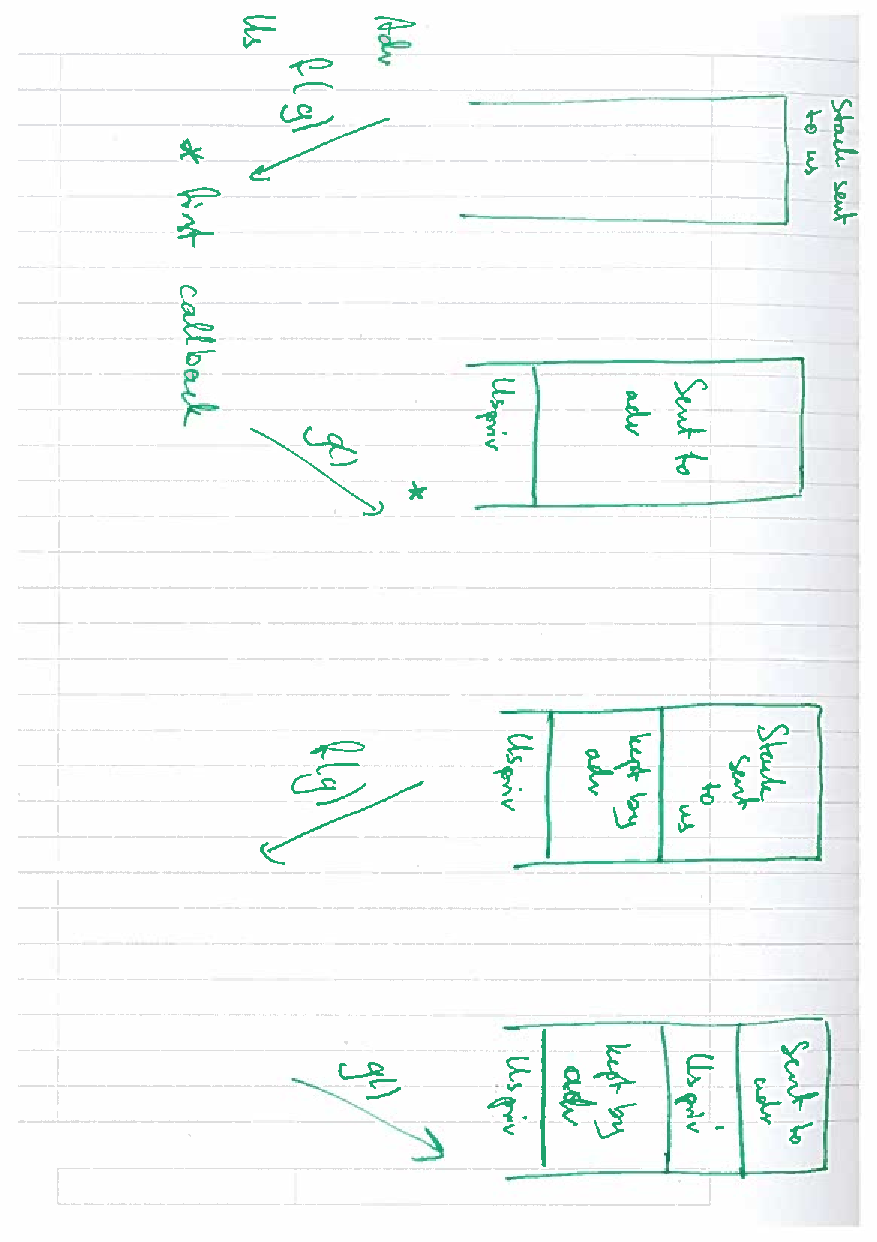
\includegraphics[angle=90,width=\textwidth]{img/ret-full-stk.pdf}
  \caption{Illustration of the stack in the example that illustrates why the entire stack must be returned.}
  \label{fig:ret-full-stk}
\end{figure}

\subsubsection{Restriction on stack allocation}
We need to somehow make sure that it is always the same stack that is used. If we don't, then an adversary can simply split the stack in two, use one part for one call and the other for another call. At this point, they can return to either of the two calls - in other words, well-bracketedness is not enforced.

\begin{itemize}
  \item An adversary starts the execution. They split the stack in two and call us with one part (say the top part) along with a callback.
  \item We use part of the stack and call the adversary with the rest of the stack.
  \item The adversary calls us again this time using the other part of the stack (here the bottom part of the stack).
  \item Again, we use part of the stack and call the adversary with the rest of this part of the stack.
\end{itemize}
At this point, the adversary can return from either of the two calls. Swapping around the order in which the adversary uses the two parts of the stack changes nothing.

The example is illustrated in Figure~\ref{fig:stk-alloc}.

One way to solve this problem is to make the "top address" of the stack known. There are many ways to do this, but we have chosen to do the following:
\begin{itemize}
\item The stack grows downwards, so the ``last address'' of the stack is the base address of the initial stack capability.
\item The base address of the stack capability is a fixed address, so in the semantics, it will be expressed as a constant that is publicly known.
\item At some point before a call, it must be checked whether the stack we are using actually has the globally known base address (if not we must fail because we cannot trust this stack).
\item To ensure that the check is made, we require it in the semantic condition (at this moment of time not defined, so we are yet to see what it looks like).
\end{itemize}

\begin{figure}
  \centering
  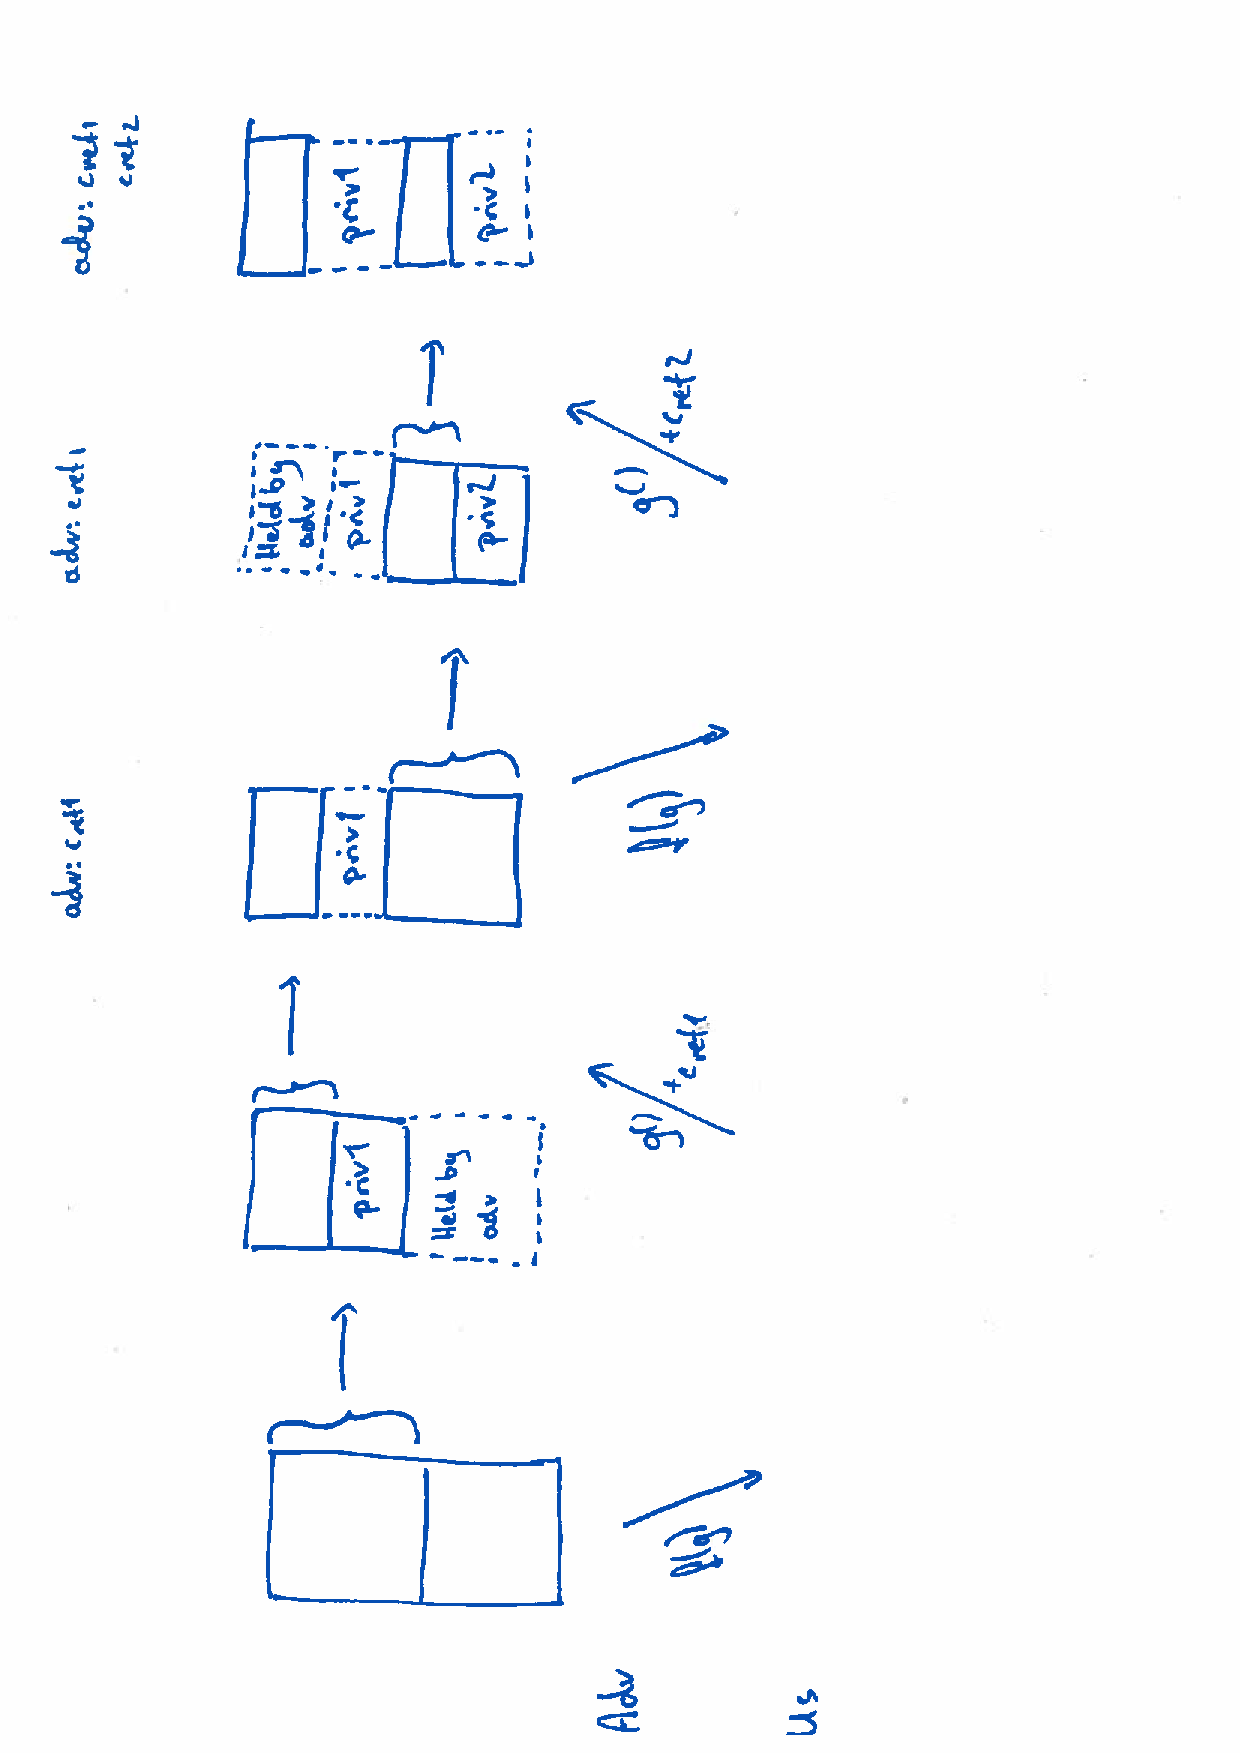
\includegraphics[angle=270,trim={0 0 5cm 0},width=\textwidth]{img/stk-alloc.pdf}
  \caption{Illustration of the potential stack allocation issue.}
  \label{fig:stk-alloc}
\end{figure}



\section{Related Work}
\subsection{Conditional Full-Abstraction}
The idea of conditional full-abstraction was used by \citet{Juglaret2016} to define full abstraction for unsafe languages. Their definition requires both the programs and the context to be fully defined (i.e.\ not cause undefined behavior). If the programs are not required to be fully-defined, then anything can happen which makes it impossible to reason about.. In our work, undefined behavior marks cases that we do not want to consider because they should be excluded further up in the compilation chain. Further, if we have to take these cases into account, then we need to add checks which protects the trusted code against itself, but properly compiled code should not have to protect itself against itself.
\lau{03-10-2017: We can adjust this when we have actually done something.}

\bibliography{references}
\end{document}